%!TEX root = ms.tex
\section{Simulation}
\label{sec:simulation}
The following three information criteria are also considered in the simulation study, that are the BIC criterion \citep{schwarz1978estimating}
\begin{equation*}
\text{BIC}(k) = n \log\left( \frac{\text{RSS}(k)}{n} \right) +\log(n) k,
%\label{eq:bic}
\end{equation*}
the generalized cross-validation (GCV) criterion \citep{craven1978smoothing}
\begin{equation*}
\text{GCV}(k) = \text{RSS}(k)\frac{n^2}{(n-k)^2},
%\label{eq:gcv_subsetselection}
\end{equation*}
and 
\begin{equation*}
\tilde{\text{C}}_p(k) = \text{RSS}(k)\frac{n+k}{n-k}.
%\label{eq:cptilde}
\end{equation*}
BIC$(k)$ is a consistent criterion, in the sense that under some conditions, if the true model is among the candidate models, the probability of selecting the true model approaches one. GCV$(k)$ is closely related to S$_p(k)$ where both are multiplicative criteria and have similar penalty terms, although GCV was derived in a different context. Recall that S$_p(k)$ is derived from $\widehat{\text{ErrR}}_\text{SE}(k)$ by plugging in the estimator $\hat\sigma_0^2 = \text{RSS}(k)/(n-k)$ based on the OLS fit on the $k$ predictors in the subset. The same procedure can be performed in the fixed-X scenario, and by plugging $\hat\sigma_0^2 = \text{RSS}(k)/(n-k)$ into $\widehat{\text{ErrR}}_\text{SE}(k)$, we obtain the expression of $\tilde{\text{C}}_p(k)$. Furthermore, by analogy to the criteria discussed in Section \ref{sec:ic_fixedx} and \ref{sec:ic_randomx}, we substitute $k=p-m$ into the expressions of BIC$(k)$, GCV$(k)$ and $\tilde{\text{C}}_p(k)$, and we obtain their corresponding expressions for general linear restrictions which are denoted as BIC$(R,r)$, GCV$(R,r)$ and $\tilde{\text{C}}_p(R,r)$, respectively. Furthermore, we consider two types of the cross-validation (CV), that are the 10-fold CV (denoted as 10FCV) and leave-one-out CV (LOOCV). The LOOCV is based on the PRESS(k) statistic for variable selection problem and PRESS(R,r) for general restriction problem.

In this section, we start from the variable selection problem. The candidate models include the predictors of $X$ in a nested fashion, i.e. the model with size $k$ has the first $k$ columns of $X$ ($X_1,\cdots,X_k$). We further consider general restrictions on $\beta$. The conclusion is that the AICc and RAICc provide the best predictive performances regardless the designs of $X$, for both variable selection and general restriction problems.  

\subsection{Setup}
\label{sec:simulation_setup_subset}
For the variable selection problem, we consider the following configurations of the experiment.
\begin{itemize}
	\item Sample size: $n \in \{40, 200, 1000\}$.
	\item Number of predictors: $p \in \{12, n/2, n-4\}$.
	\item Correlation of predictors: $\rho \in \{0,0.5,0.9\}$.
	\item Signal level: low, medium and high. The average oracle $R^2$ (linear regression on the set of true predictors) corresponding to these three signal levels are roughly $20\%$, $50\%$ and $90\%$, respectively.
	\item The correlation structure $\Sigma_0$ (entries are $\sigma_{0,ij}$ where $\sigma_{0,ii}=1$ for $i=1,\cdots,p$) and true coefficient vector $\beta_0$ include the following scenarios:
	\begin{itemize}
		\item Sparse-Ex1: \textbf{All of the predictors (both signal and noise) are correlated.} We take $\sigma_{0,ij}=\rho^{|i-j|}$ for $i,j\in\{1,\cdots,p\}\times\{1,\cdots,p\}$. $\beta_0=[3.5,3,2.5,2,1.5,1,0_{p-6}]^T$. 
		\item Sparse-Ex2: \textbf{Signal predictors are only correlated with signal predictors, and noise predictors are only correlated with noise predictors.} We take $\sigma_{0,ij}=\sigma_{0,ji}=\rho$ for $1\le i <j \le 6$ and $7\le i <j \le p$. Other off-diagonal elements in $\Sigma_0$ are zero. $\beta_0=[1,1,3,3,5,5,0_{p-6}]^T$.
		%\item Sparse-Ex3: \textbf{Signal predictors are pairwise correlated with noise predictors.} We take $\sigma_{0,ij}=\sigma_{0,ji}=\rho$ for $1\le i \le 6$ and $j=6+i$. Other off-diagonal elements in $\Sigma_0$ are zero. $\beta_0=[1_6,0_{p-6}]^T$.
		%\item Sparse-Ex4: \textbf{Signal predictors are pairwise correlated with opposite effects.} We take $\sigma_{0,ij}=\sigma_{0,ji}=\rho$ for $1\le i <j \le 6$. Other off-diagonal elements in $\Sigma_0$ are zero. $\beta_0=[1,-1,3,-3,5,-5,0_{p-6}]^T$.
		\item Dense-Ex1 \citep{Taddy2017}: \textbf{Same correlation structure as Sparse-Ex1, but with diminishing strengths of coefficients}. The true coefficient vector has: $\beta_{0,j} = \displaystyle (-1)^j \exp(-\frac{j}{\kappa})$, $j=1,\cdots,p$, and here $\kappa=10$.
		%\item Dense-Ex2: \textbf{Same setup as Dense-Ex1, but with slower decay}. Here we take $\kappa=50$.
	\end{itemize}
  \item Design matrix $X$: fixed-X and random-X.
\end{itemize}

For the general restriction problem, we consider the following configurations.
\begin{itemize}
  \item Sample size: $n \in \{10, 100, 500\}$.
  \item Number of predictors: $p=6$.
  \item Correlation of predictors: $\rho \in \{0,0.5,0.9\}$.
  \item Signal level: low, medium and high. The average oracle $R^2$ (linear regression on the set of true predictors) corresponding to these three signal levels are roughly $20\%$, $50\%$ and $90\%$, respectively.
  \item The entries of the covariance matrix $\Sigma_0$: $\sigma_{0,ij}=\rho^{|i-j|}$ for $i,j\in\{1,\cdots,p\}\times\{1,\cdots,p\}$.
  \item The true coefficient vector:
  \begin{itemize}
    \item Ex1: $\beta_0 = [2,2,2,1,1,1]^T$. 
    \item Ex2: $\beta_0 = [-2,2,2,-1.5,-1.5,1]^T$.
    \item Ex3: $\beta_0 = [2,-2,1,-1,0.5,-0.5]^T$.
  \end{itemize}
  \item Restrictions:
  \begin{itemize}
    \item Ex1: 
    \begin{itemize}
      \item Correct: $\beta_1=\beta_2$, $\beta_2=\beta_3$, $\beta_4=\beta_5$, $\beta_5=\beta_6$, $\beta_1=2\beta_4$
      \item Wrong: $\beta_1=\beta_4$, $\beta_2=\beta_5$, $\beta_3=\beta_6$, $\beta_1=2\beta_2$, $\beta_2=2\beta_3$
    \end{itemize}
    \item Ex2:
    \begin{itemize}
      \item Correct: $\beta_1=-\beta_2$, $\beta_1=-\beta_3$, $\beta_3=2\beta_6$, $\beta_4=\beta_5$, $\beta_3+\beta_4+\beta_5+\beta_6=0$
      \item Wrong: $\beta_5=-\beta_6$, $\beta_4=-\beta_6$, $\beta_4=2\beta_1$, $\beta_1=\beta_2$, $\beta_1+\beta_2+\beta_3+\beta_4=0$
    \end{itemize}
    \item Ex3: 
    \begin{itemize}
      \item Correct: $\beta_1=-\beta_2$, $\beta_3=-\beta_4$, $\beta_5=-\beta_6$, $\beta_1=2\beta_3$, $\beta_3=2\beta_5$
      \item Wrong: $\beta_1=-\beta_4$, $\beta_2=-\beta_5$, $\beta_3=-\beta_6$, $\beta_1=2\beta_2$, $\beta_2=2\beta_3$
    \end{itemize}
    For each example, we have a series of correct and wrong restrictions, where the correct restrictions are the ones that hold for the choice of $\beta_0$. The candidate restriction set is considered by combining all the possible combinations of restrictions in the correct series and all the possible combinations of those in the wrong series. We also consider the null model (restricting all coefficients to be zero) and the full model (no restriction). In total, we have $64$ candidate restrictions.
  \end{itemize}
  \item Design matrix $X$: fixed-X and random-X.
\end{itemize}


For the random-X scenario, in each replication, we generate an $X$ where the rows $x_i$ ($i=1,\cdots,n$) are drawn from a $p$-dimensional multivariate normal distribution with mean zero and covariance matrix $\Sigma_0$, and we draw the response $y$ from the conditional distribution of $y|X$ based on \eqref{eq:truemodel}. The entire process is repeated $1000$ times. For the fixed-X scenario, we only generate $X$ once and draw $1000$ replications of $y$ based on the same $X$ and \eqref{eq:truemodel}. We consider the following metrics to evaluate the fit.
\begin{itemize}
	\item Squared error loss (on log scale):
	\begin{equation*}
  \begin{aligned}
		\text{loglossF} &= \log\left( \frac{1}{n}\lVert X\hat{\beta} - X\beta_0 \rVert_2^2 \right).\\
    \text{loglossR} &= \log\left( E_{X^n} \lVert X^n\hat\beta-X^n\beta_0 \rVert_2^2 \right) = \log\left( (\hat{\beta}-\beta_0)^T \Sigma_0 (\hat{\beta}-\beta_0) \right).
  \end{aligned}
	\end{equation*}
  loglossF and loglossR are the fixed-X and random-X versions of the loss on the log scale, respectively. 
  \iffalse
	\item Relative risk:
	\begin{equation*}
		\text{RR}(\hat{\beta}) = \frac{E_{X^n} \lVert X^n\hat\beta-X^n\beta_0 \rVert_2^2}{E_{X^n} \lVert X^n\beta_0 \rVert_2^2} = \frac{(\hat{\beta}-\beta_0)^T \Sigma_0 (\hat{\beta}-\beta_0)}{\beta_0^T \Sigma_0 \beta_0}.
	\end{equation*}
	\item Relative test error:
	\begin{equation*}
		\text{RTE}(\hat{\beta}) = \frac{E_{X^n,y^n} \lVert y^n - X^n\hat\beta \rVert_2^2}{\sigma_0^2}= \frac{(\hat{\beta}-\beta_0)^T \Sigma_0 (\hat{\beta}-\beta_0) + \sigma_0^2}{\sigma_0^2}.
	\end{equation*}
	\item Proportion of variance explained: 
	\begin{equation*}
		\text{PVE}(\hat{\beta}) = 1 - \frac{E_{X^n,y^n} \lVert y^n- X^n\hat\beta \rVert_2^2}{\text{Tr}\left( \text{Cov}_{y^n} (y^n) \right)}= 1-\frac{(\hat{\beta}-\beta_0)^T \Sigma_0 (\hat{\beta}-\beta_0)+\sigma_0^2}{\beta_0^T \Sigma_0 \beta_0 + \sigma_0^2}.
	\end{equation*}
  \fi
	\item KL discrepancy (on log scale): logKLF and logKLR are the fixed-X and random-X versions of the KL on the log scale, where the expressions KL are given in \eqref{eq:KLF} and \eqref{eq:KLR}, respectively.
  \iffalse
  \begin{equation*}
  \begin{aligned}
    \text{KLF} &= \text{KLF}(\hat\beta)  \\
    %&= \log\left( \frac{n\log(2\pi\lVert y-X\hat\beta \rVert_2^2 /n) + n\lVert X\hat{\beta} - X\beta_0 \rVert_2^2/\lVert y-X\hat\beta \rVert_2^2+n^2 \sigma_0^2 / \lVert y-X\hat\beta \rVert_2^2}{n\log(2\pi\lVert y \rVert_2^2 /n) + n\lVert X\beta_0 \rVert_2^2/\lVert y \rVert_2^2+n^2 \sigma_0^2 / \lVert y \rVert_2^2} \right).\\
    \text{KLR} &= \text{KLR}(\hat\beta) 
    %&= \log\left(\frac{n\log(2\pi\lVert y-X\hat\beta \rVert_2^2 /n) + n^2 (\hat{\beta}-\beta_0)^T \Sigma_0 (\hat{\beta}-\beta_0)/\lVert y-X\hat\beta \rVert_2^2+n^2 \sigma_0^2 / \lVert y-X\hat\beta \rVert_2^2}{n\log(2\pi\lVert y \rVert_2^2 /n) + n^2 \beta_0^T \Sigma_0 \beta_0/\lVert y \rVert_2^2+n^2 \sigma_0^2 / \lVert y \rVert_2^2} \right).
  \end{aligned}
  \end{equation*}
  \fi
  %Note that $\widetilde{\text{ErrR}}$ is obtained ErrR, by removing the terms that do not change when we compare two models ($np\log(2\pi)$, $n\log|\hat{\Sigma}|$ and $n\text{Tr}(\hat\Sigma^{-1}\Sigma_{0})$). We find that for large $n$ and $p$, these terms dominate the values of ErrR, and make it hard to differentiate the performances of two models as they appear in the criteria of both models. 
	\item Size of the subset selected for the variable selection problem, and number of restrictions given by the selected model for the general restriction problem.
\end{itemize}
There are in total $486$ scenarios for the variable selection problem, and $162$ scenarios for the general restriction problem. The full set of simulation results is presented in the Supplemental Material. 

\iffalse
\subsubsection{Without a true model}
\begin{itemize}
	\item Omit: The configuration is the same as Sparse-Ex1, but with the 6-th predictor treated as missing for all the fitting procedures.
	\item Exponential: We take $\Sigma = I$. The responses are generated by $y_i=exp(4i/n) + \epsilon_i$, for $i=1,\cdots,n$, where $\epsilon_i$ are independent $\mathcal{N}(0, \sigma_0^2)$. 
\end{itemize}
	We consider a fixed trigonometric configuration of $X$ that is studied by \citet{Hurvich1991}, where $X$ is an $n$ by $p$ matrix with components defined by 
$$ x_{t, 2j-1} = \sin\left(\frac{2\pi j}{n}t\right),$$
and 
$$ x_{t,2j} = \cos\left(\frac{2\pi j}{n}t\right),$$
for $j=1,\cdots,p/2$ and $t=0,\cdots,n-1$. The responses are generated by $y_i=exp(4i/n) + \epsilon_i$, for $i=1,\cdots,n$, where $\epsilon_i$ are independent $\mathcal{N}(0, \sigma_0^2)$. 
\fi


\subsection{Results for random-X}
For the variable selection problem, we find that RAICc provides the best predictive performance and the sparsest subset, compared to other selection rules designed for random-X, including RC$_p$, S$_p$ and LOO CV. For example, we see from \ref{fig:subsetselection_randomx_hsnr_largep} and \ref{fig:subsetselection_randomx_lsnr_largep} that, RAICc performs the best with the sample size $n$ being both small and close to the dimension $p$. The only exception is when the true model is dense and the signal is high, where S$_p$ and LOO CV are better in terms of the squared loss, while RAICc is better in terms of KL. The underperformance of S$_p$ and LOO CV is result from the selection of large subsets in some of the replications. When the sample size $n$ is large, S$_p$, LOO CV and RAICc exhibit similar performances. RC$_p$ is always outperformed by the other three selection rules, regardless of the sample size. The price of estimating $\sigma_0$ as opposed to knowing it, is obvious. We also notice that the selection rules designed for random-X generally perform better than their partners for the fixed-X case. Both C$_p$ and $\tilde{\text{C}}_p$ are largely outperformed by RC$_p$ and S$_p$, respectively. The advantage of RAICc over AICc is statistically significant in most scenarios, based on the Wilcoxon signed-rank test, but is not obvious in a practical sense. Finally, we note some other findings that have been discussed in the existing literatures. BIC has a high chance to select the full model when $n$ is close to $p$, and the overfitting issue of BIC was discussed in \citet{baraud2009gaussian}. We also see that GCV performs largely the same compared to S$_p$, due to the similarity of their penalty terms. 10-fold CV performs slightly better than LOO CV especially when $n$ is small. \citet{zhang2015cross} showed that when applied as selection rules, the larger validation set given by 10-fold CV can better distinguish the candidates and results in a better model. 

In a related study by \citet{leeb2008evaluation}, the author showed that S$_p$ and GCV outperform AICc under the random-X design. We find that his results are not directly comparable to ours. First, all of his results are based on estimating a squared error-based testing error, while AICc is estimating the KL-based testing error. As we noted that, the squared error-based metric can lead to different conclusions compared to KL. Also, in the simulation studies, the author did not consider the case where $p$ is close to $n$, which in our opinion is exactly the scenario that separates the performances of various criteria. 

For the general restriction problem, we see from Figure \ref{fig:generalrestriction_randomx} that RAICc is the best selection rule for small sample size $n$, and it is the second to the best for large $n$ where it is outperformed by BIC. We also notice a clear advantage of RAICc over AICc when $n$ is small. Therefore, RAICc is a favorable selection rule for both variable selection and general restriction problems, under the random-X.

\textcolor{red}{Some discussions regarding multiplicative penalty vs additive penalty?}

\iffalse
\begin{figure}[!ht]
  \centering
  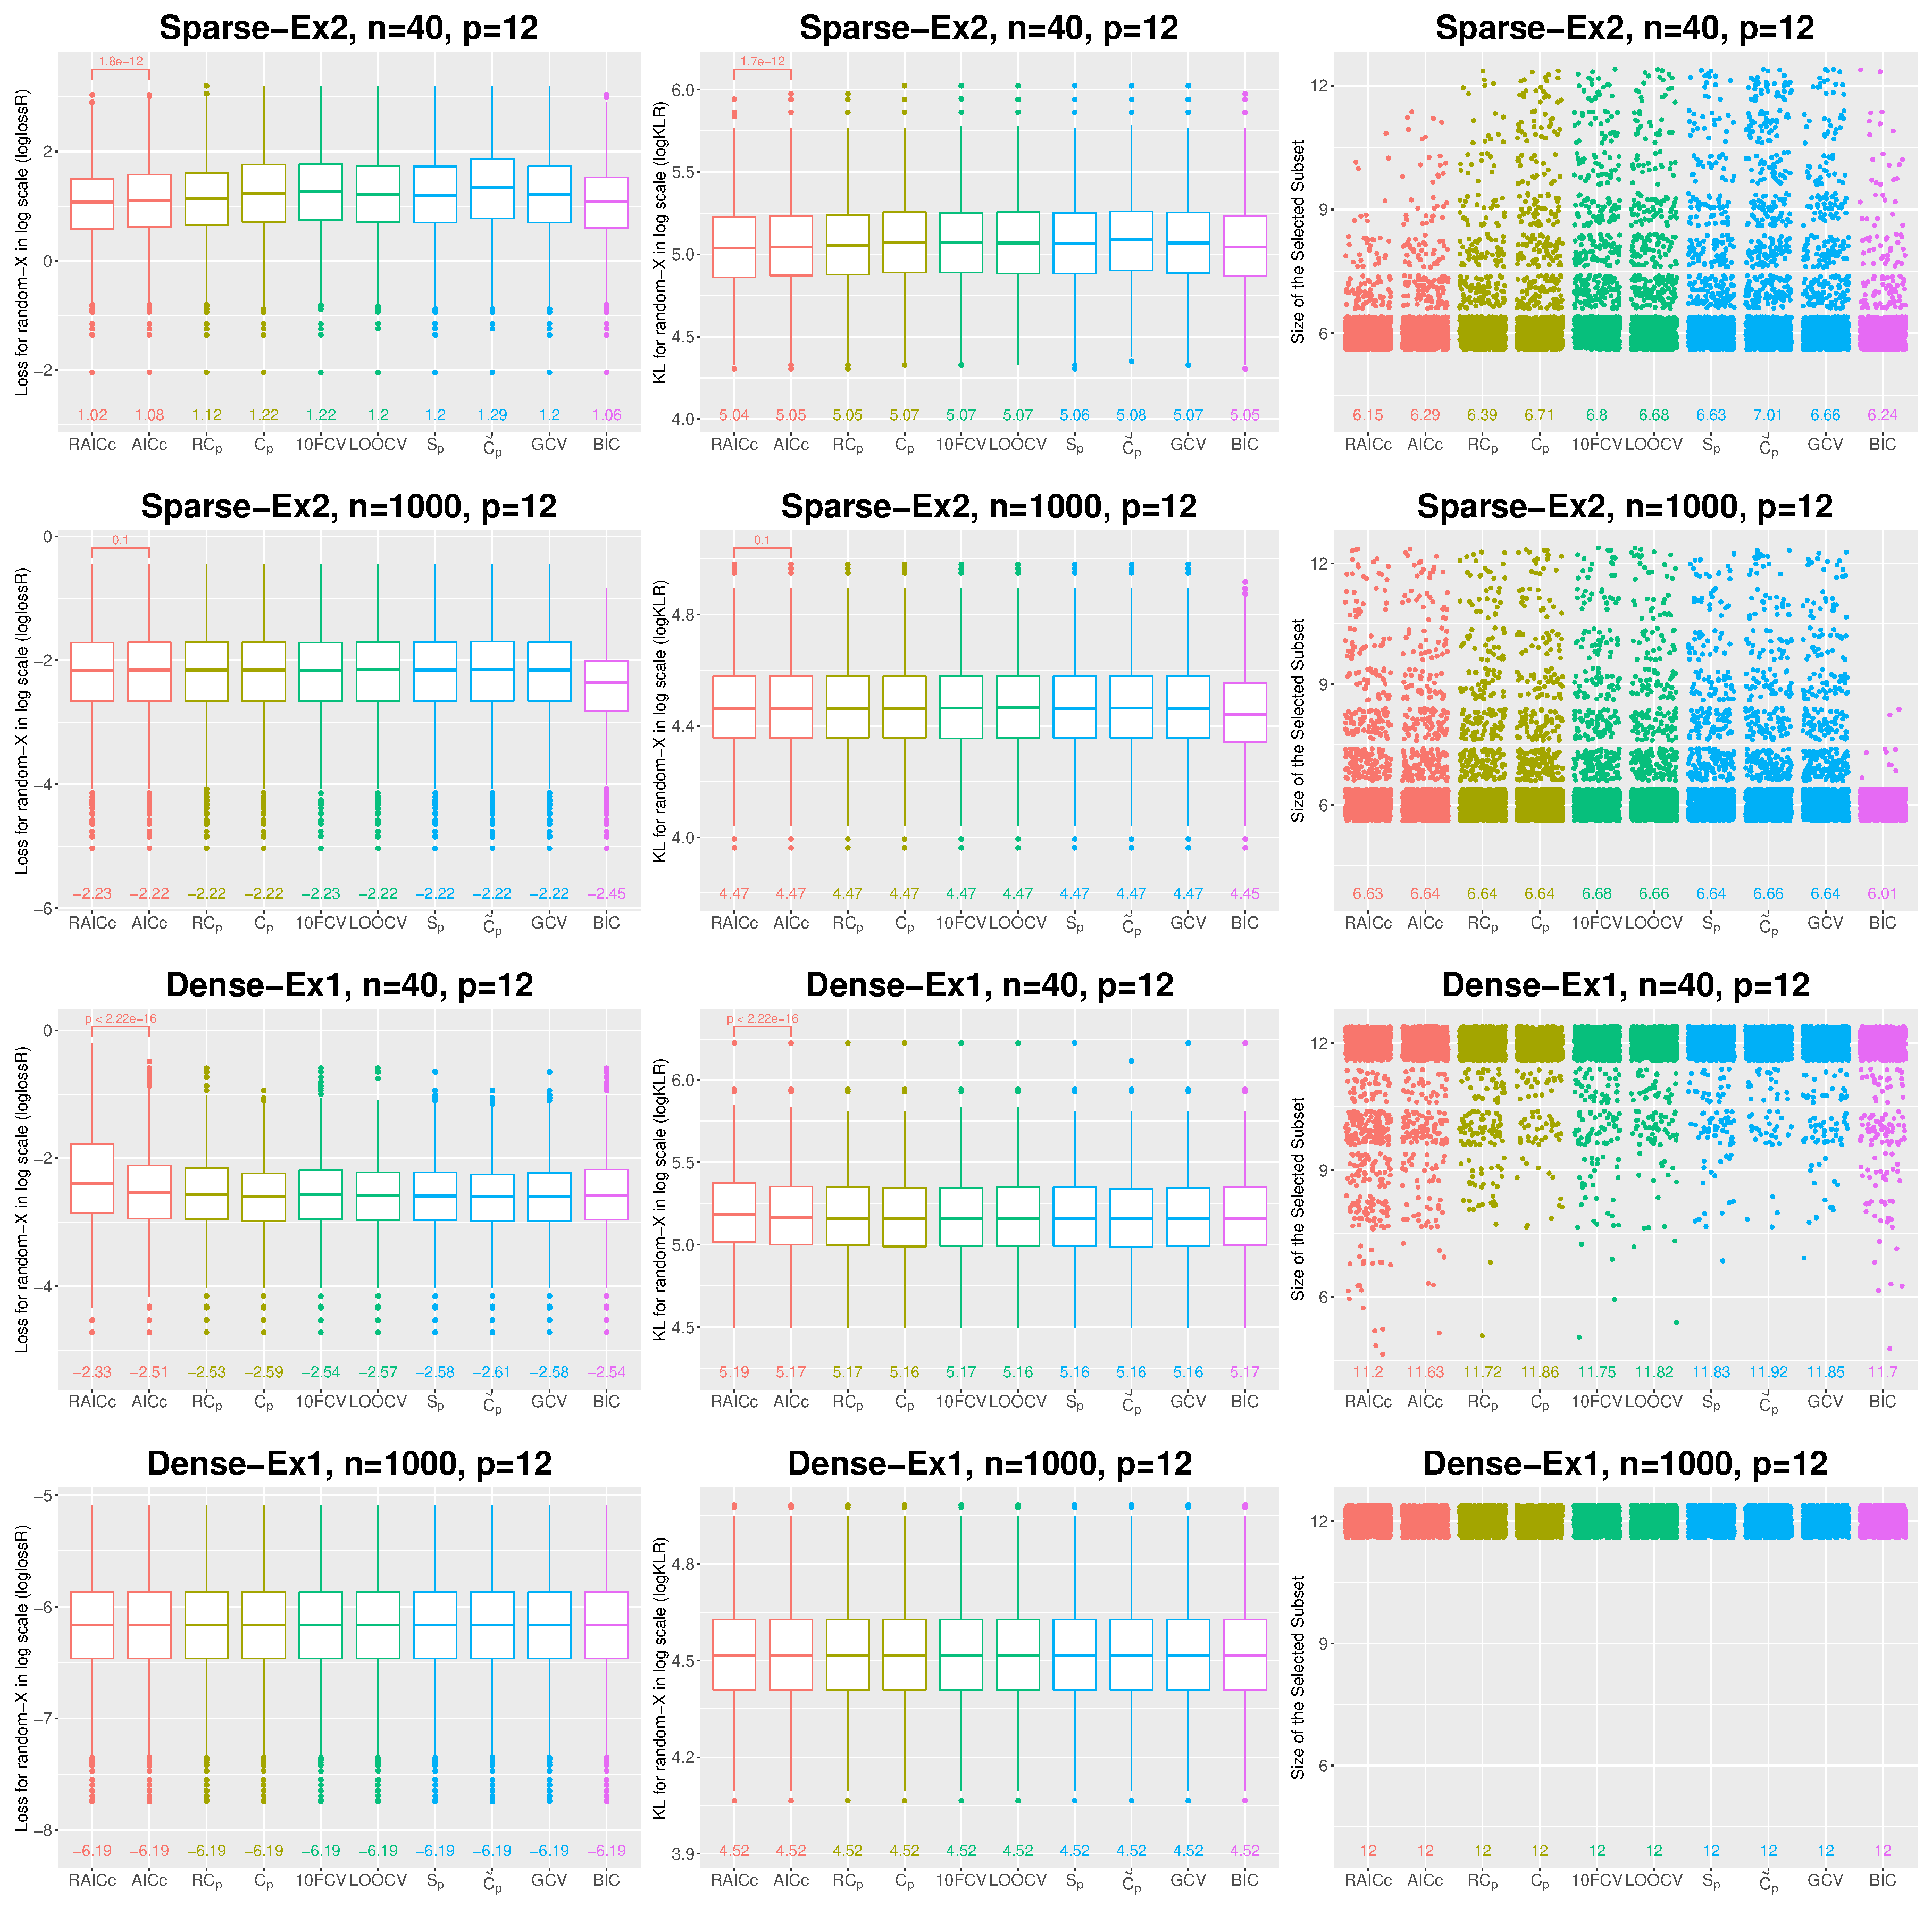
\includegraphics[width=\textwidth]{figures/main/randomx/subset_selection/smallp_hsnr.eps}
  \caption{Random-X, high signal and $\rho=0.5$. The mean values of the evaluation metrics for each criterion are presented at the bottom of each graph. The p-values of the Wilcoxon signed-rank test (paired and two-sided) for comparing RAICc and AICc are also presented.}
  \label{fig:subsetselection_randomx_hsnr_smallp}
\end{figure}

\begin{figure}[!ht]
  \centering
  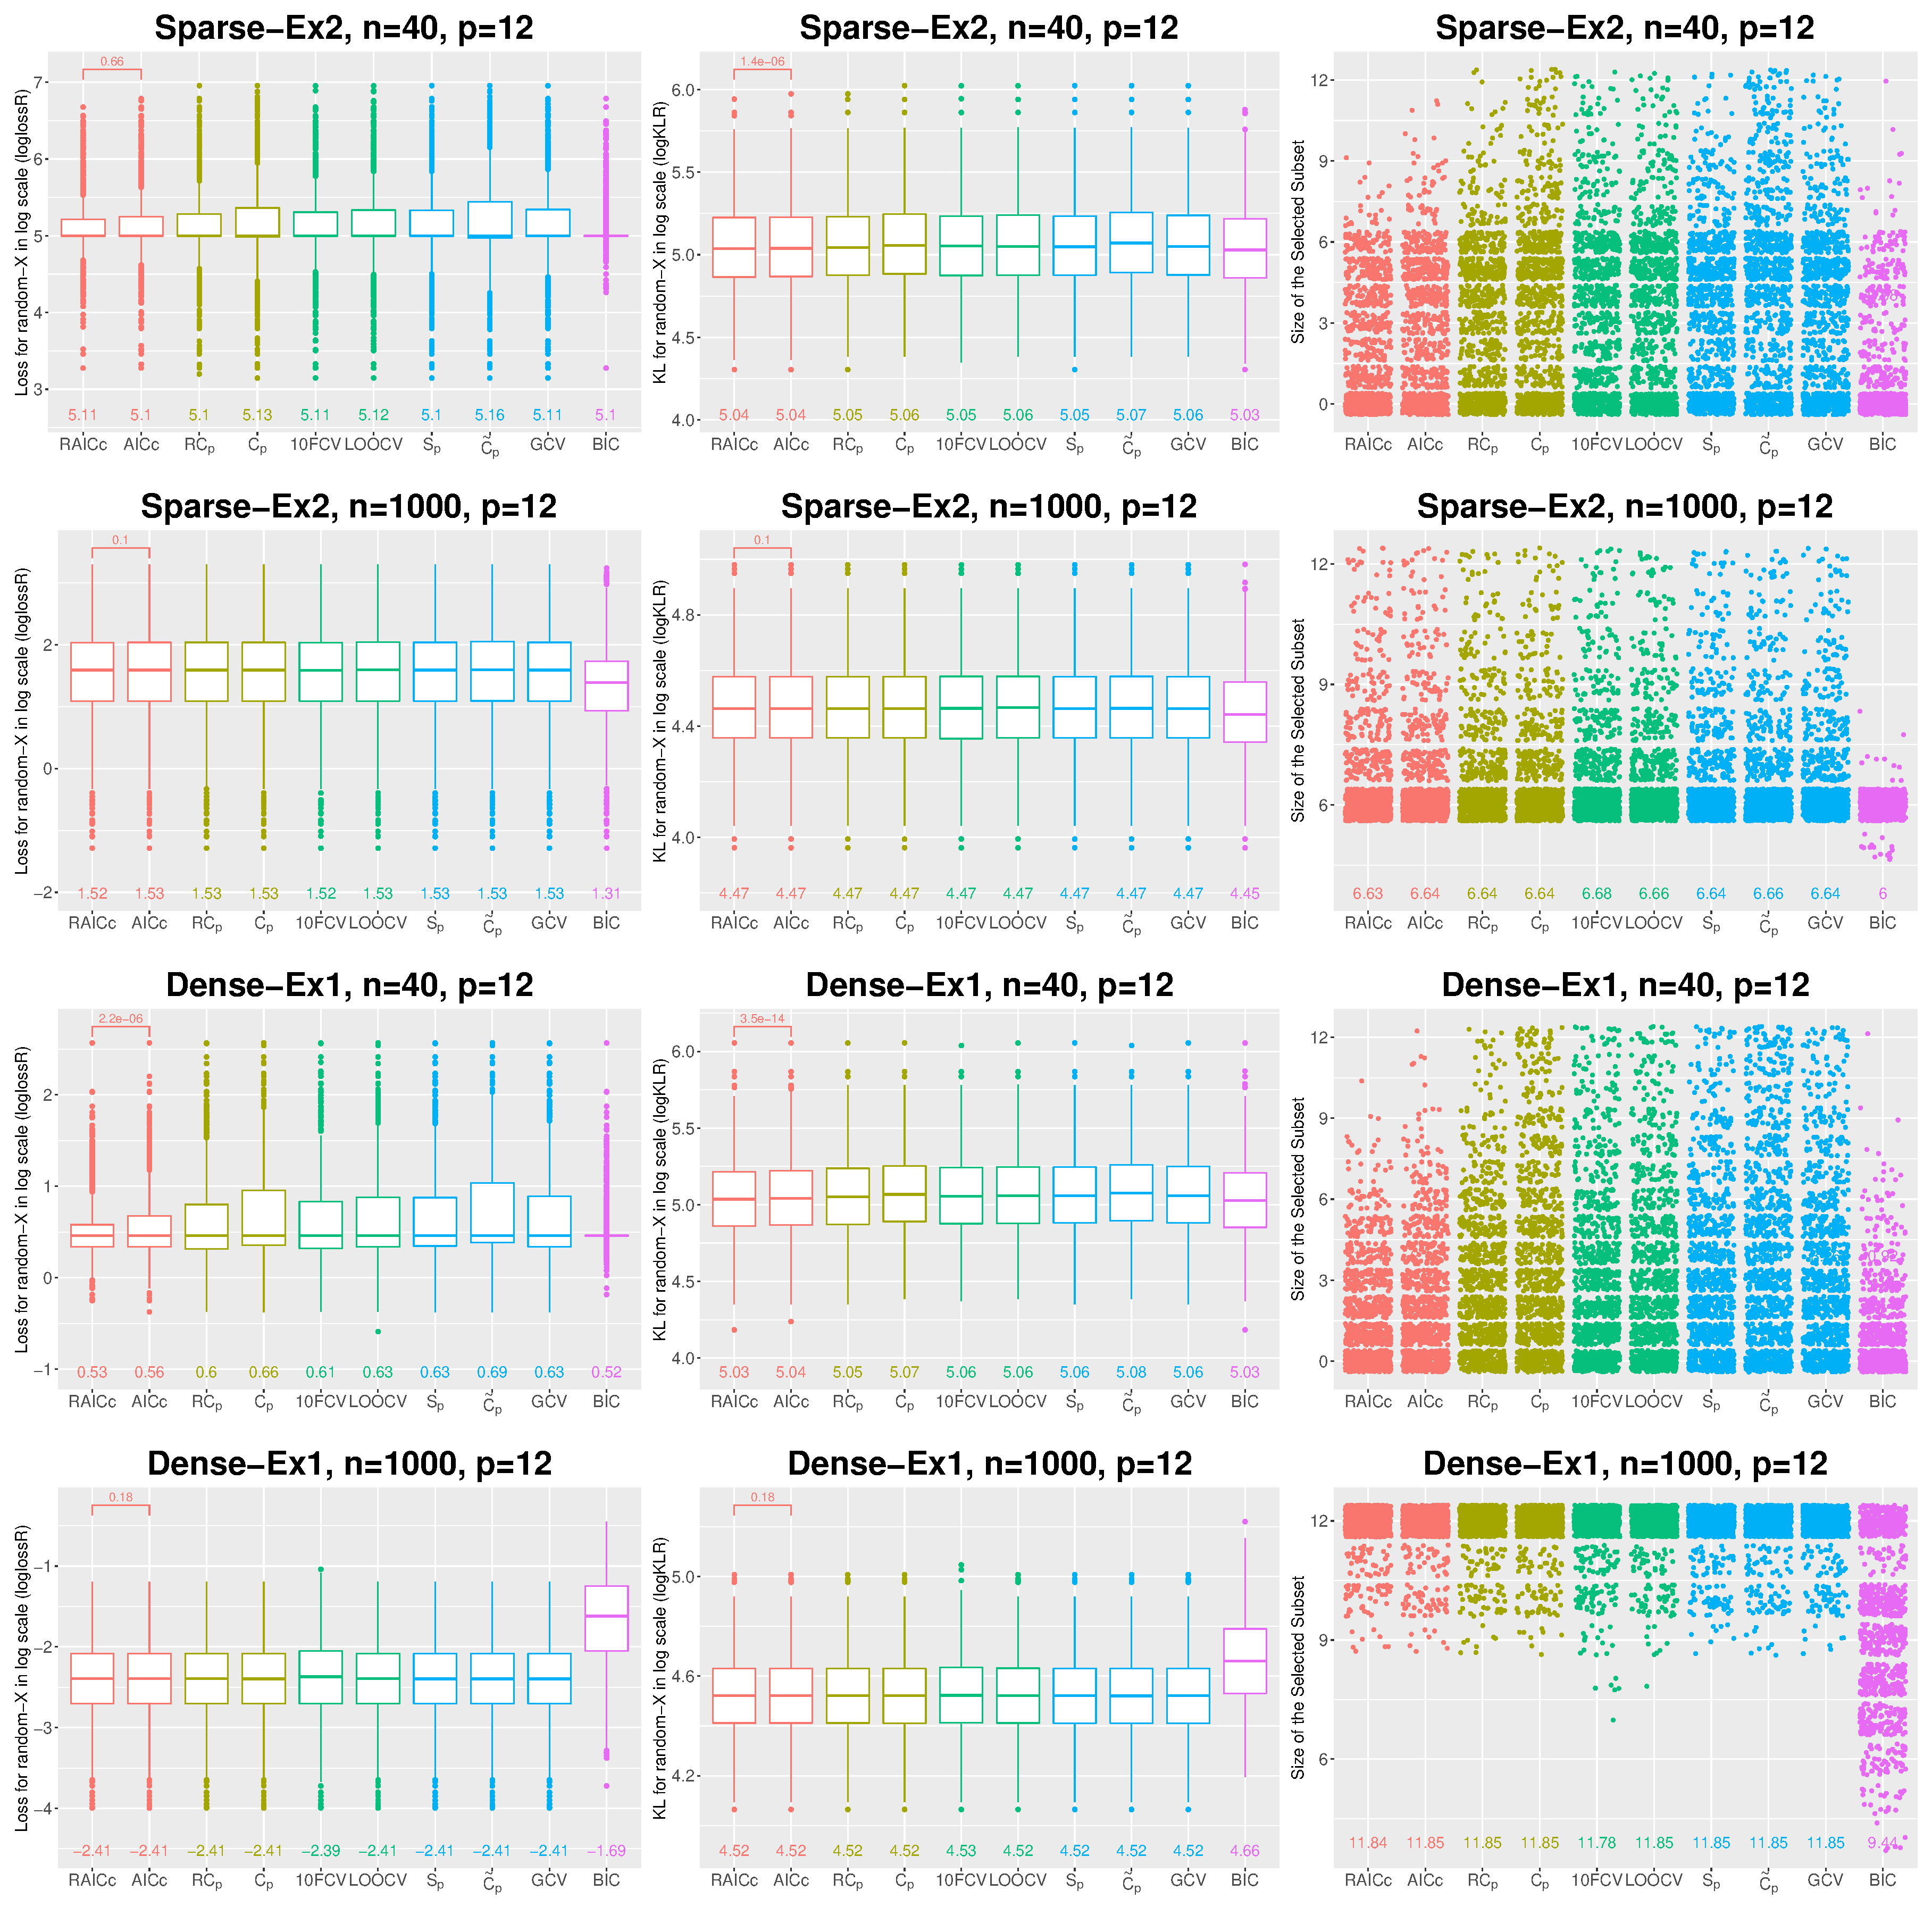
\includegraphics[width=\textwidth]{figures/main/randomx/subset_selection/smallp_lsnr.eps}
  \caption{Random-X, low signal and $\rho=0.5$. Other details are the same as in Figure \ref{fig:randomx_hsnr_smallp}.}
  \label{fig:subsetselection_randomx_lsnr_smallp}
\end{figure}
\fi

\begin{figure}[!ht]
  \centering
  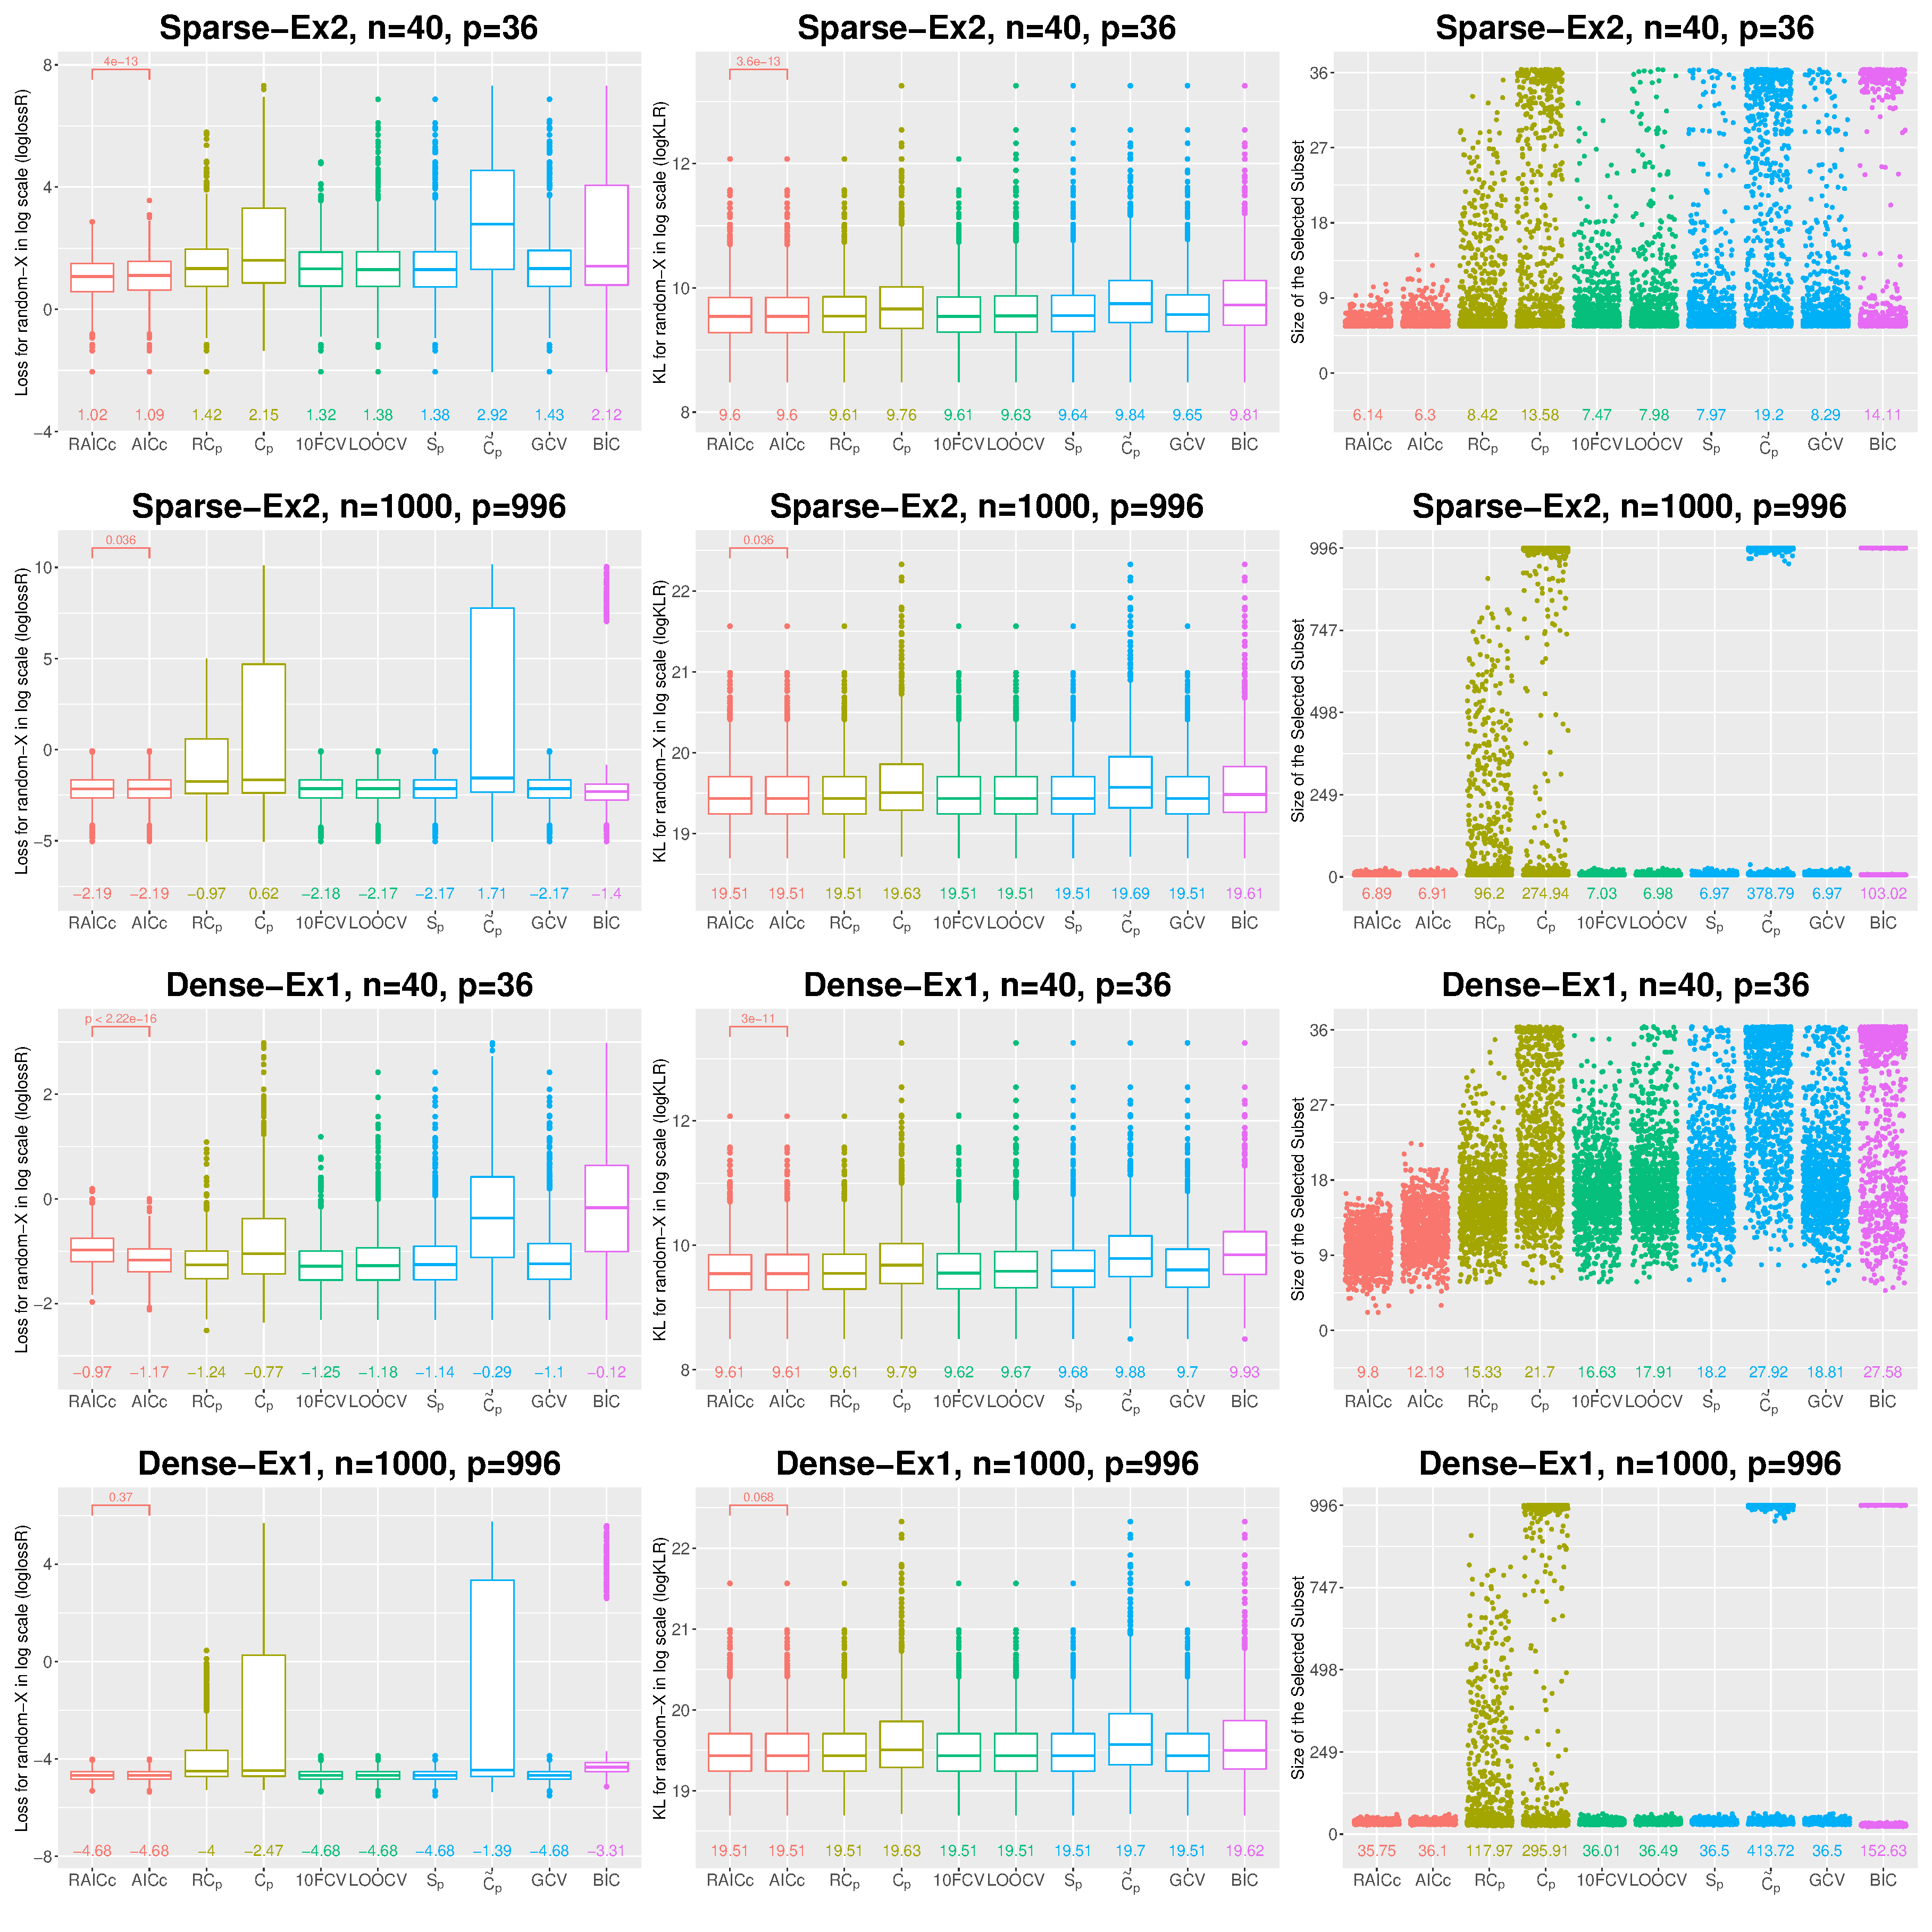
\includegraphics[width=\textwidth]{figures/main/randomx/subset_selection/largep_hsnr.eps}
  \caption{Random-X, high signal and $\rho=0.5$. The mean values of the evaluation metrics for each criterion are presented at the bottom of each graph. The p-values of the Wilcoxon signed-rank test (paired and two-sided) for comparing RAICc and AICc are also presented.}
  \label{fig:subsetselection_randomx_hsnr_largep}
\end{figure}


\begin{figure}[!ht]
  \centering
  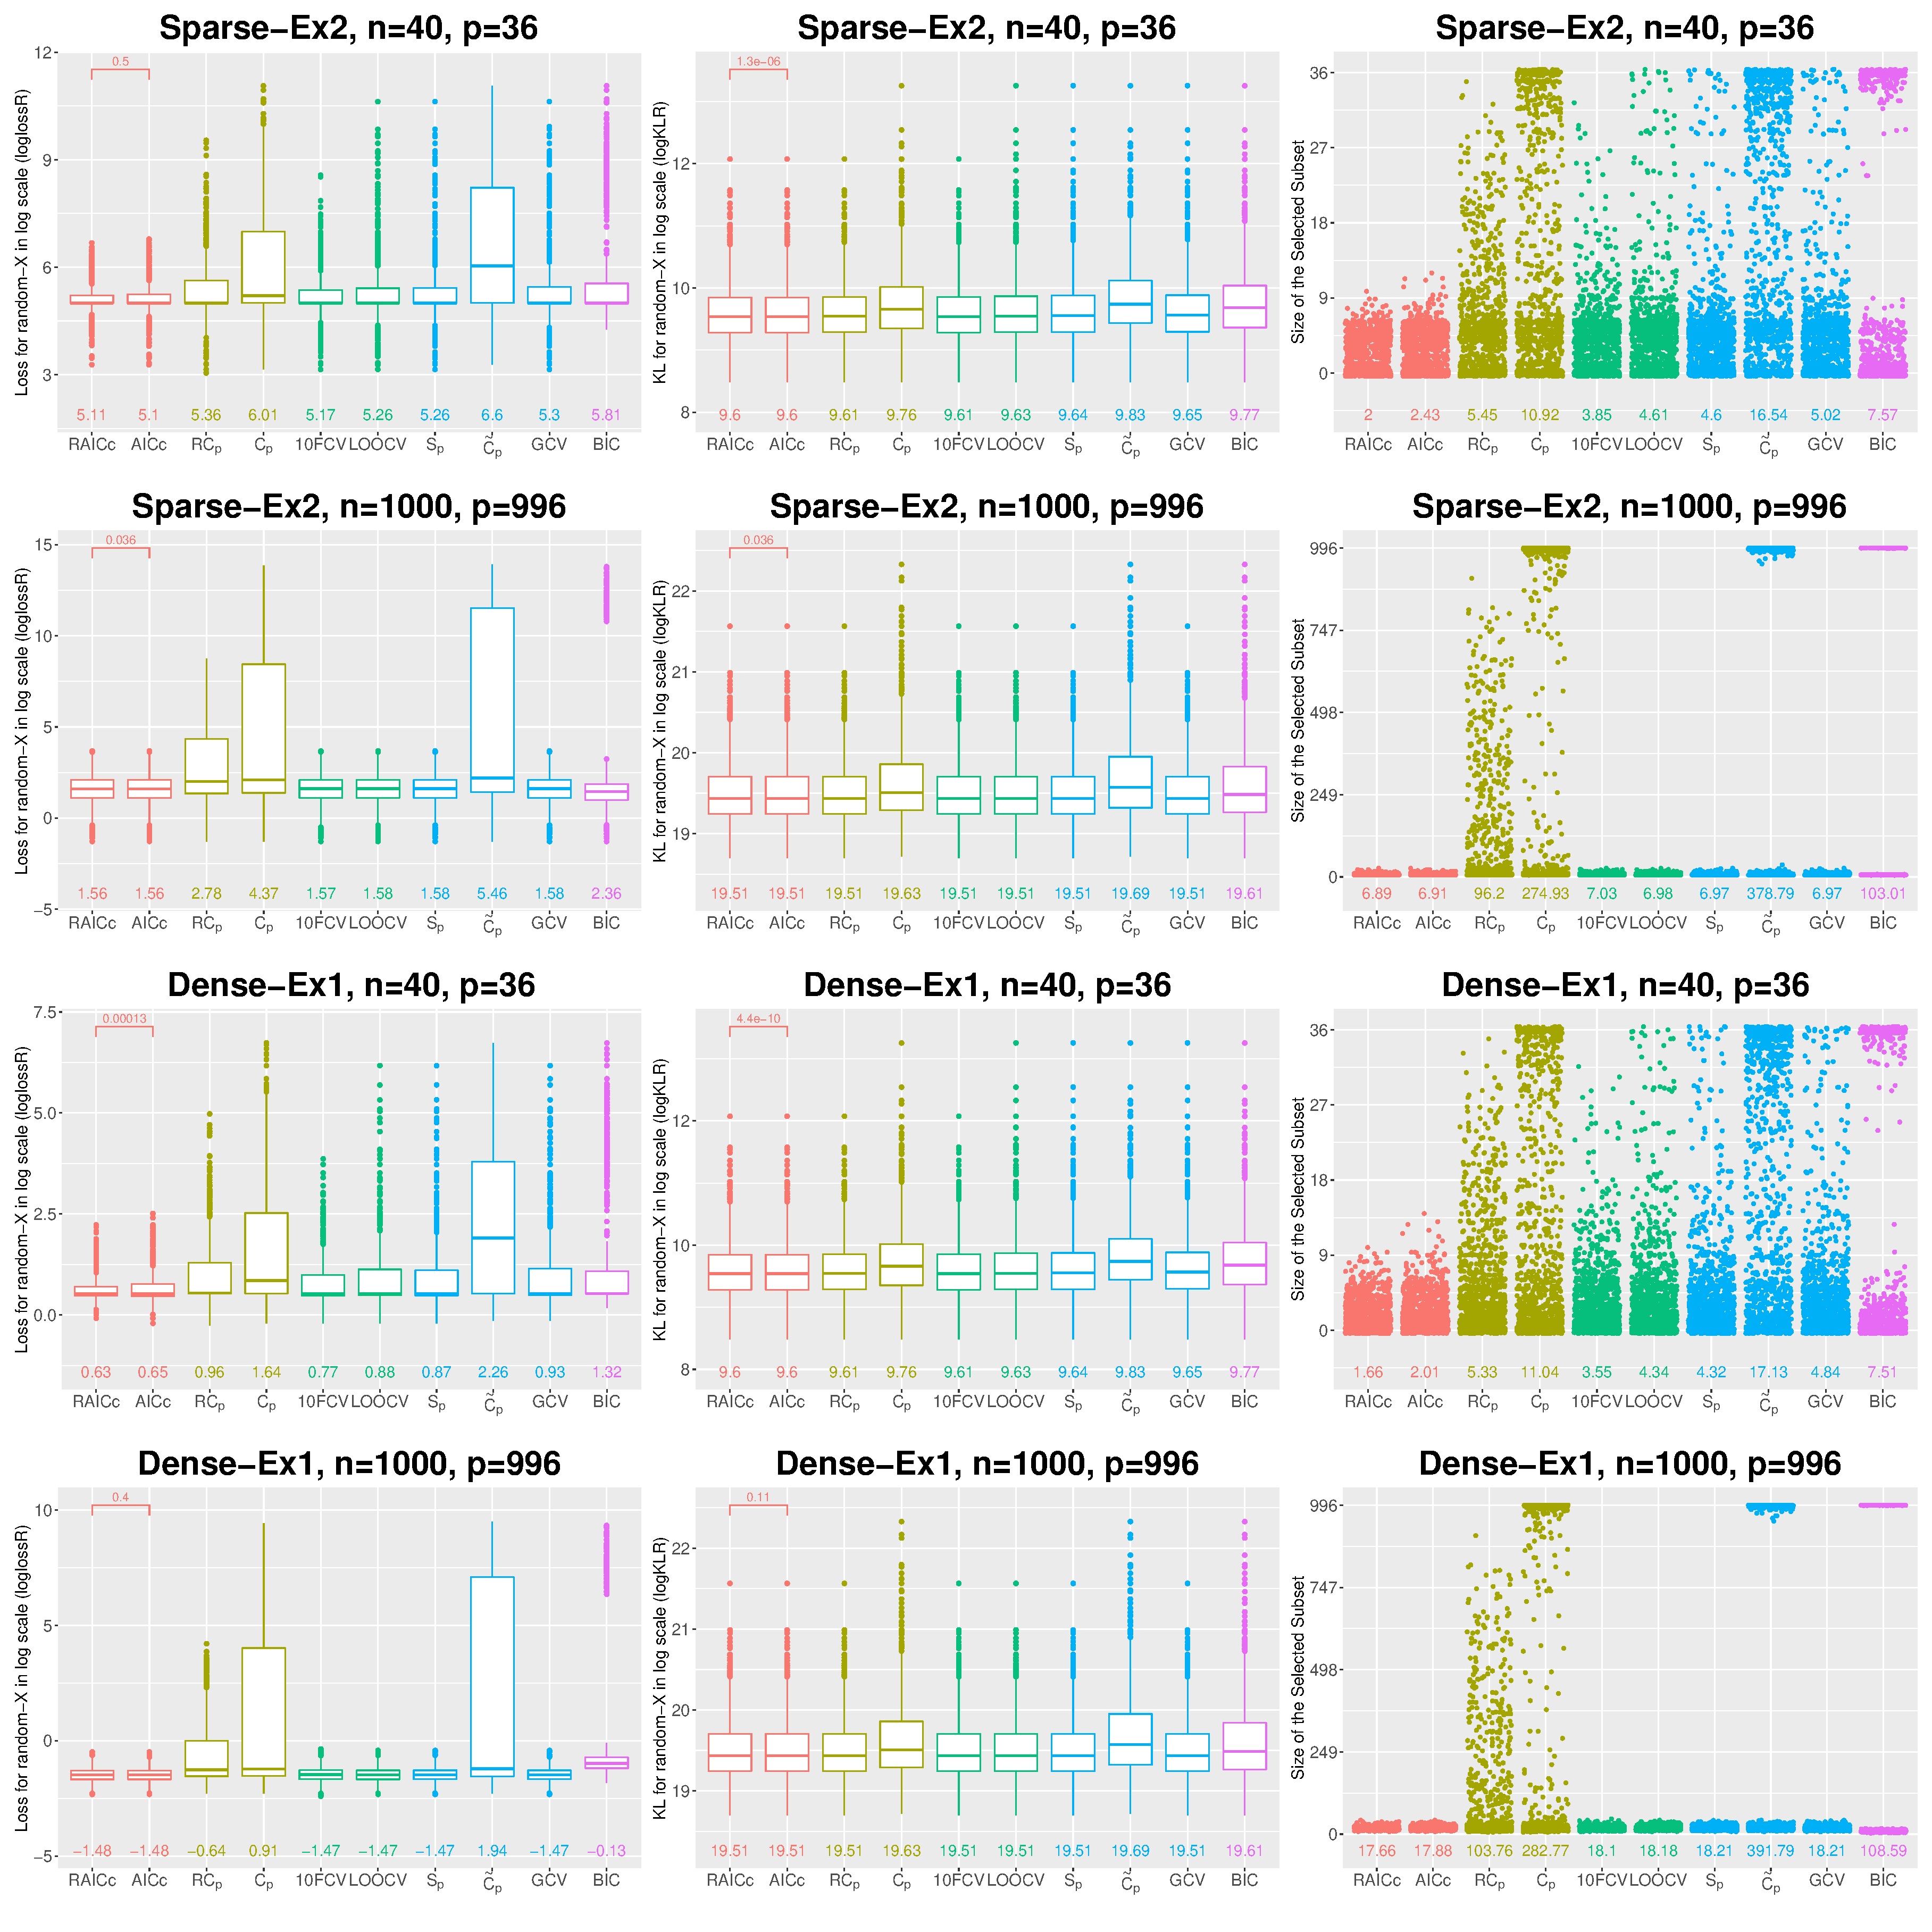
\includegraphics[width=\textwidth]{figures/main/randomx/subset_selection/largep_lsnr.eps}
  \caption{Random-X, low signal and $\rho=0.5$. The mean values of the evaluation metrics for each criterion are presented at the bottom of each graph. The p-values of the Wilcoxon signed-rank test (paired and two-sided) for comparing RAICc and AICc are also presented.}
  \label{fig:subsetselection_randomx_lsnr_largep}
\end{figure}

\begin{figure}[!ht]
  \centering
  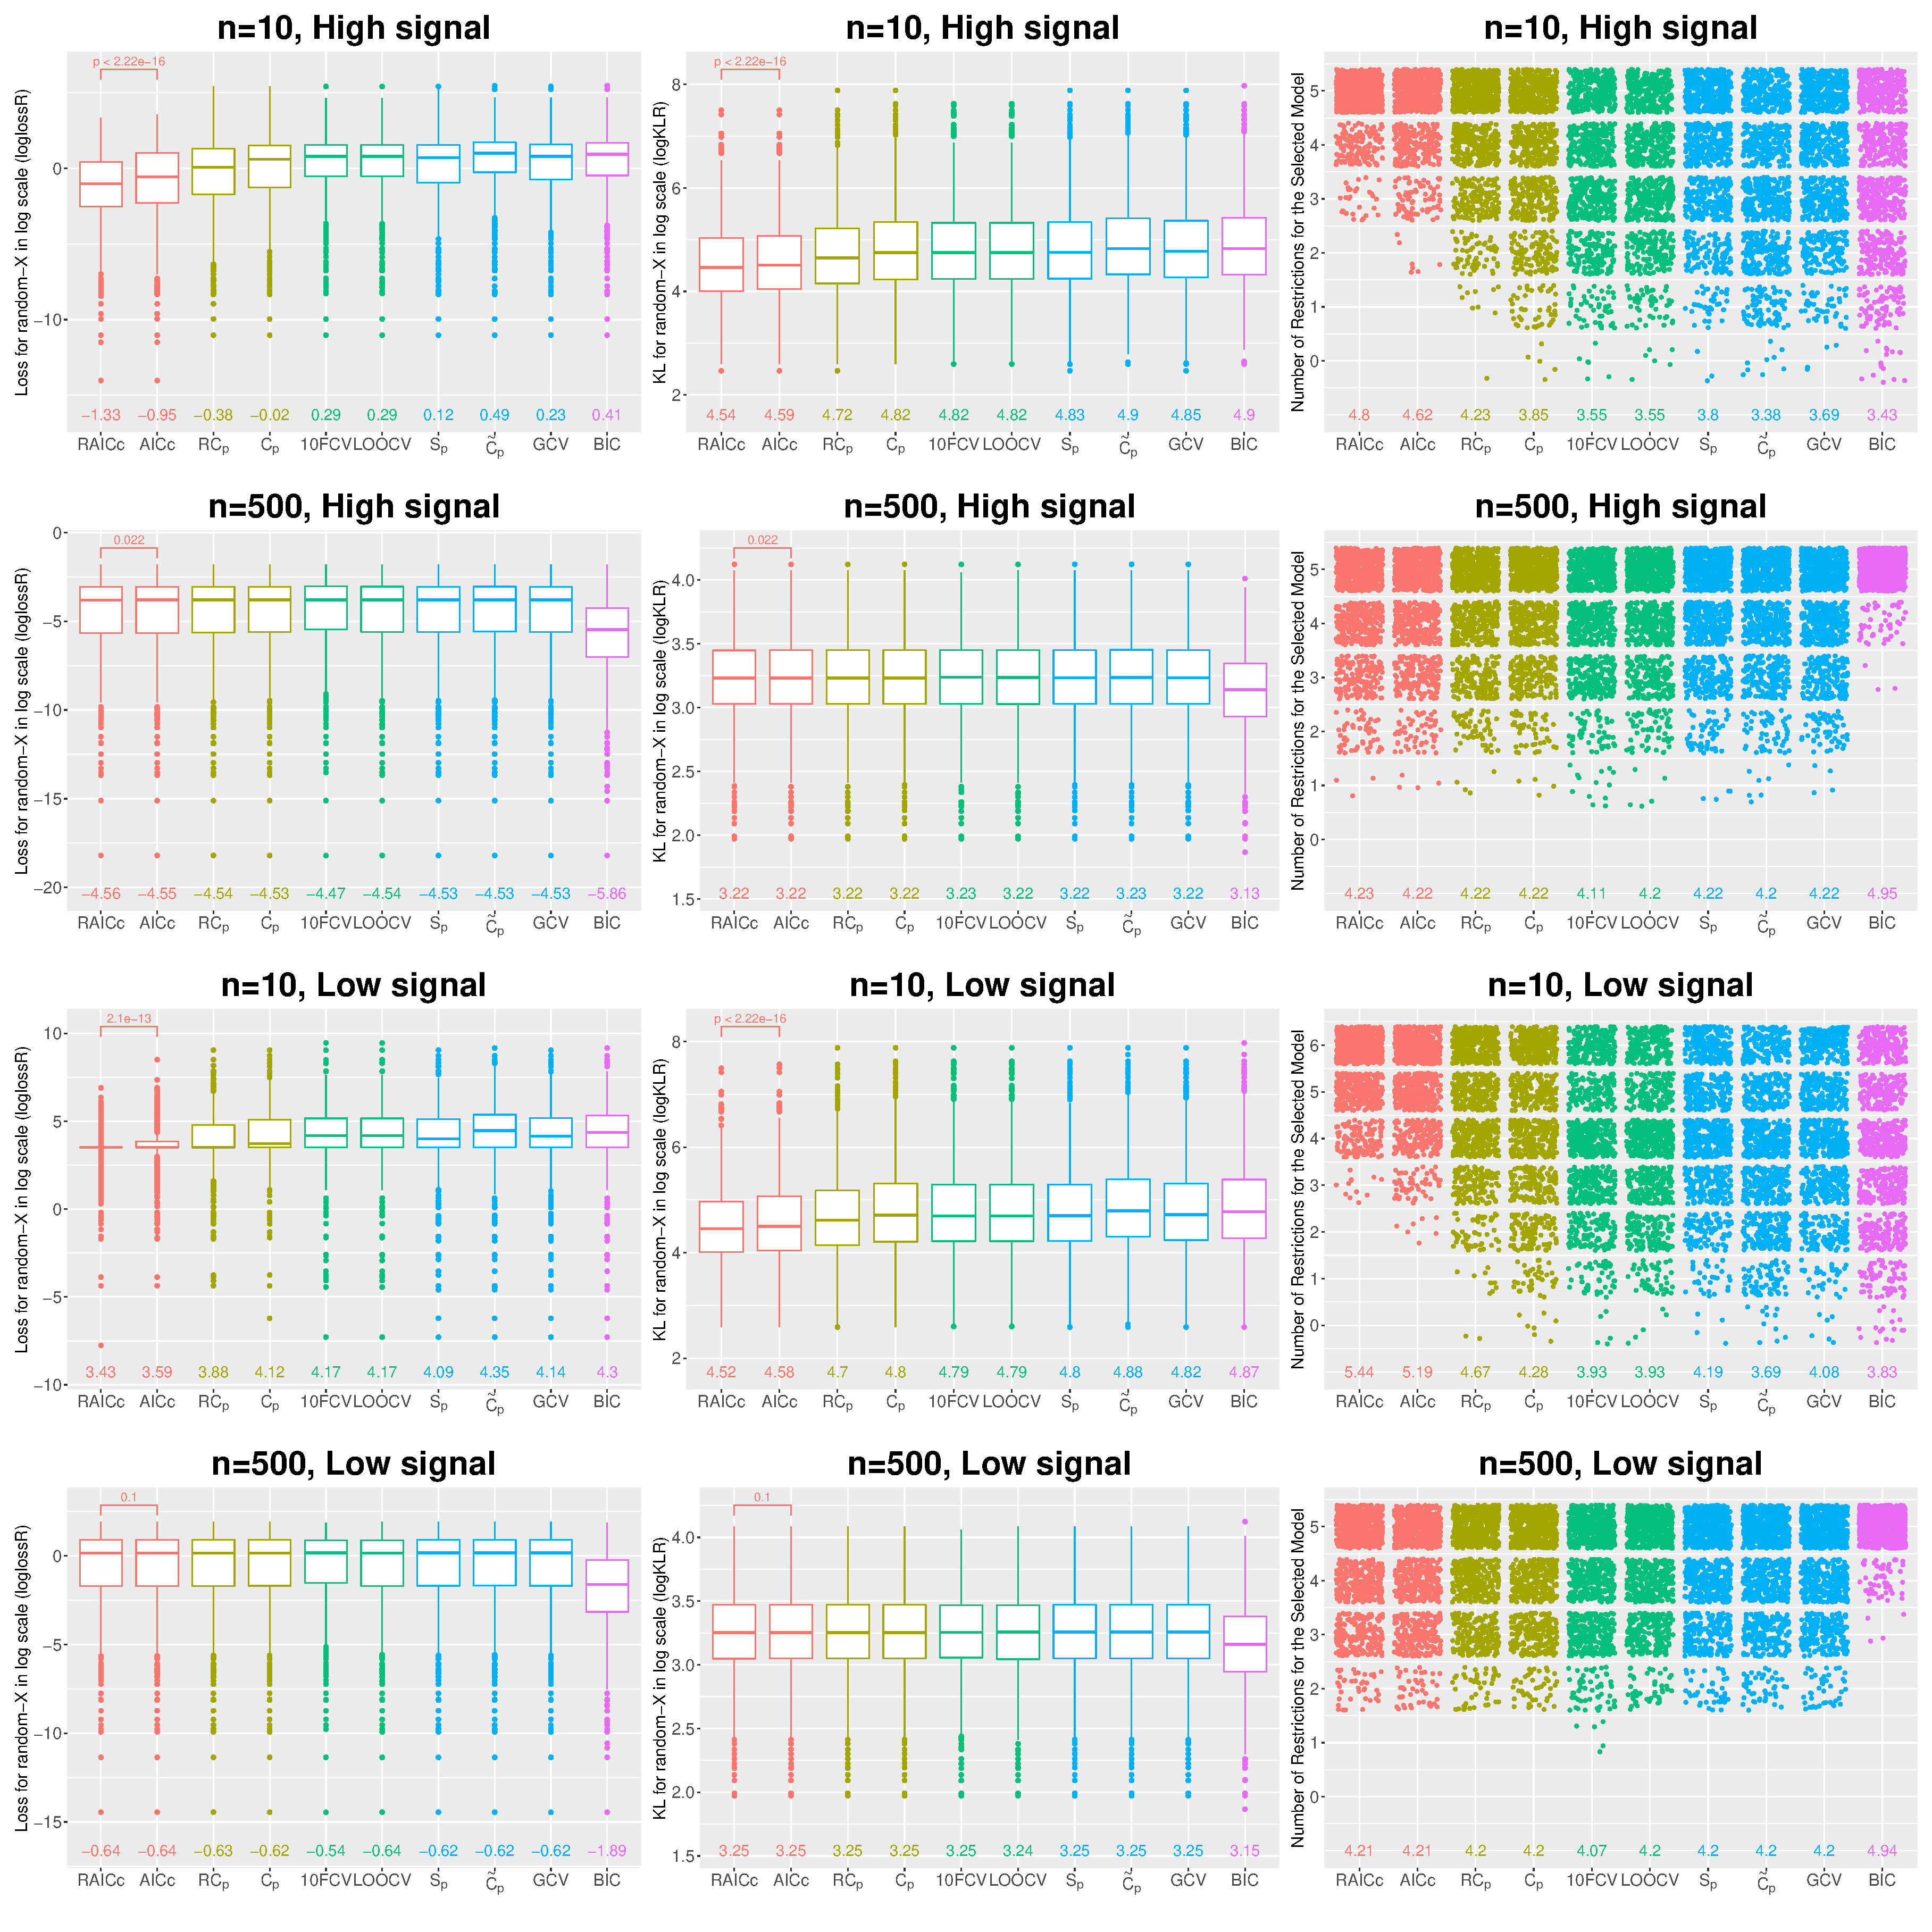
\includegraphics[width=\textwidth]{figures/main/randomx/general_restriction/Ex1.eps}
  \caption{Random-X, Ex1, $p=6$, $\rho=0.5$. The mean values of the evaluation metrics for each criterion are presented at the bottom of each graph. The p-values of the Wilcoxon signed-rank test (paired and two-sided) for comparing RAICc and AICc are also presented.}
  \label{fig:generalrestriction_randomx}
\end{figure}


\subsection{Results for fixed-X}
The comparisons of the selection rules discussed for the random-X scenario, hold for the fixed-X case as shown in Figure \ref{fig:subsetselection_fixedx_hsnr_largep}, \ref{fig:subsetselection_fixedx_lsnr_largep} and \ref{fig:generalrestriction_fixedx}. Therefore, the KL-based criteria (RAICc and AICc) are overall the best selection rules for both fixed-X and random-x designs, and RAICc has an advantage over AICc for the general restriction problem. It is surprising to see that with $X$ being fixed, selection rules designed for random-X outperform their partners for fixed-X. This may be related to the fact that providing unbiased estimates of the testing error and selecting the candidate with the best predictive performance, are different goals.  

\begin{figure}[!ht]
  \centering
  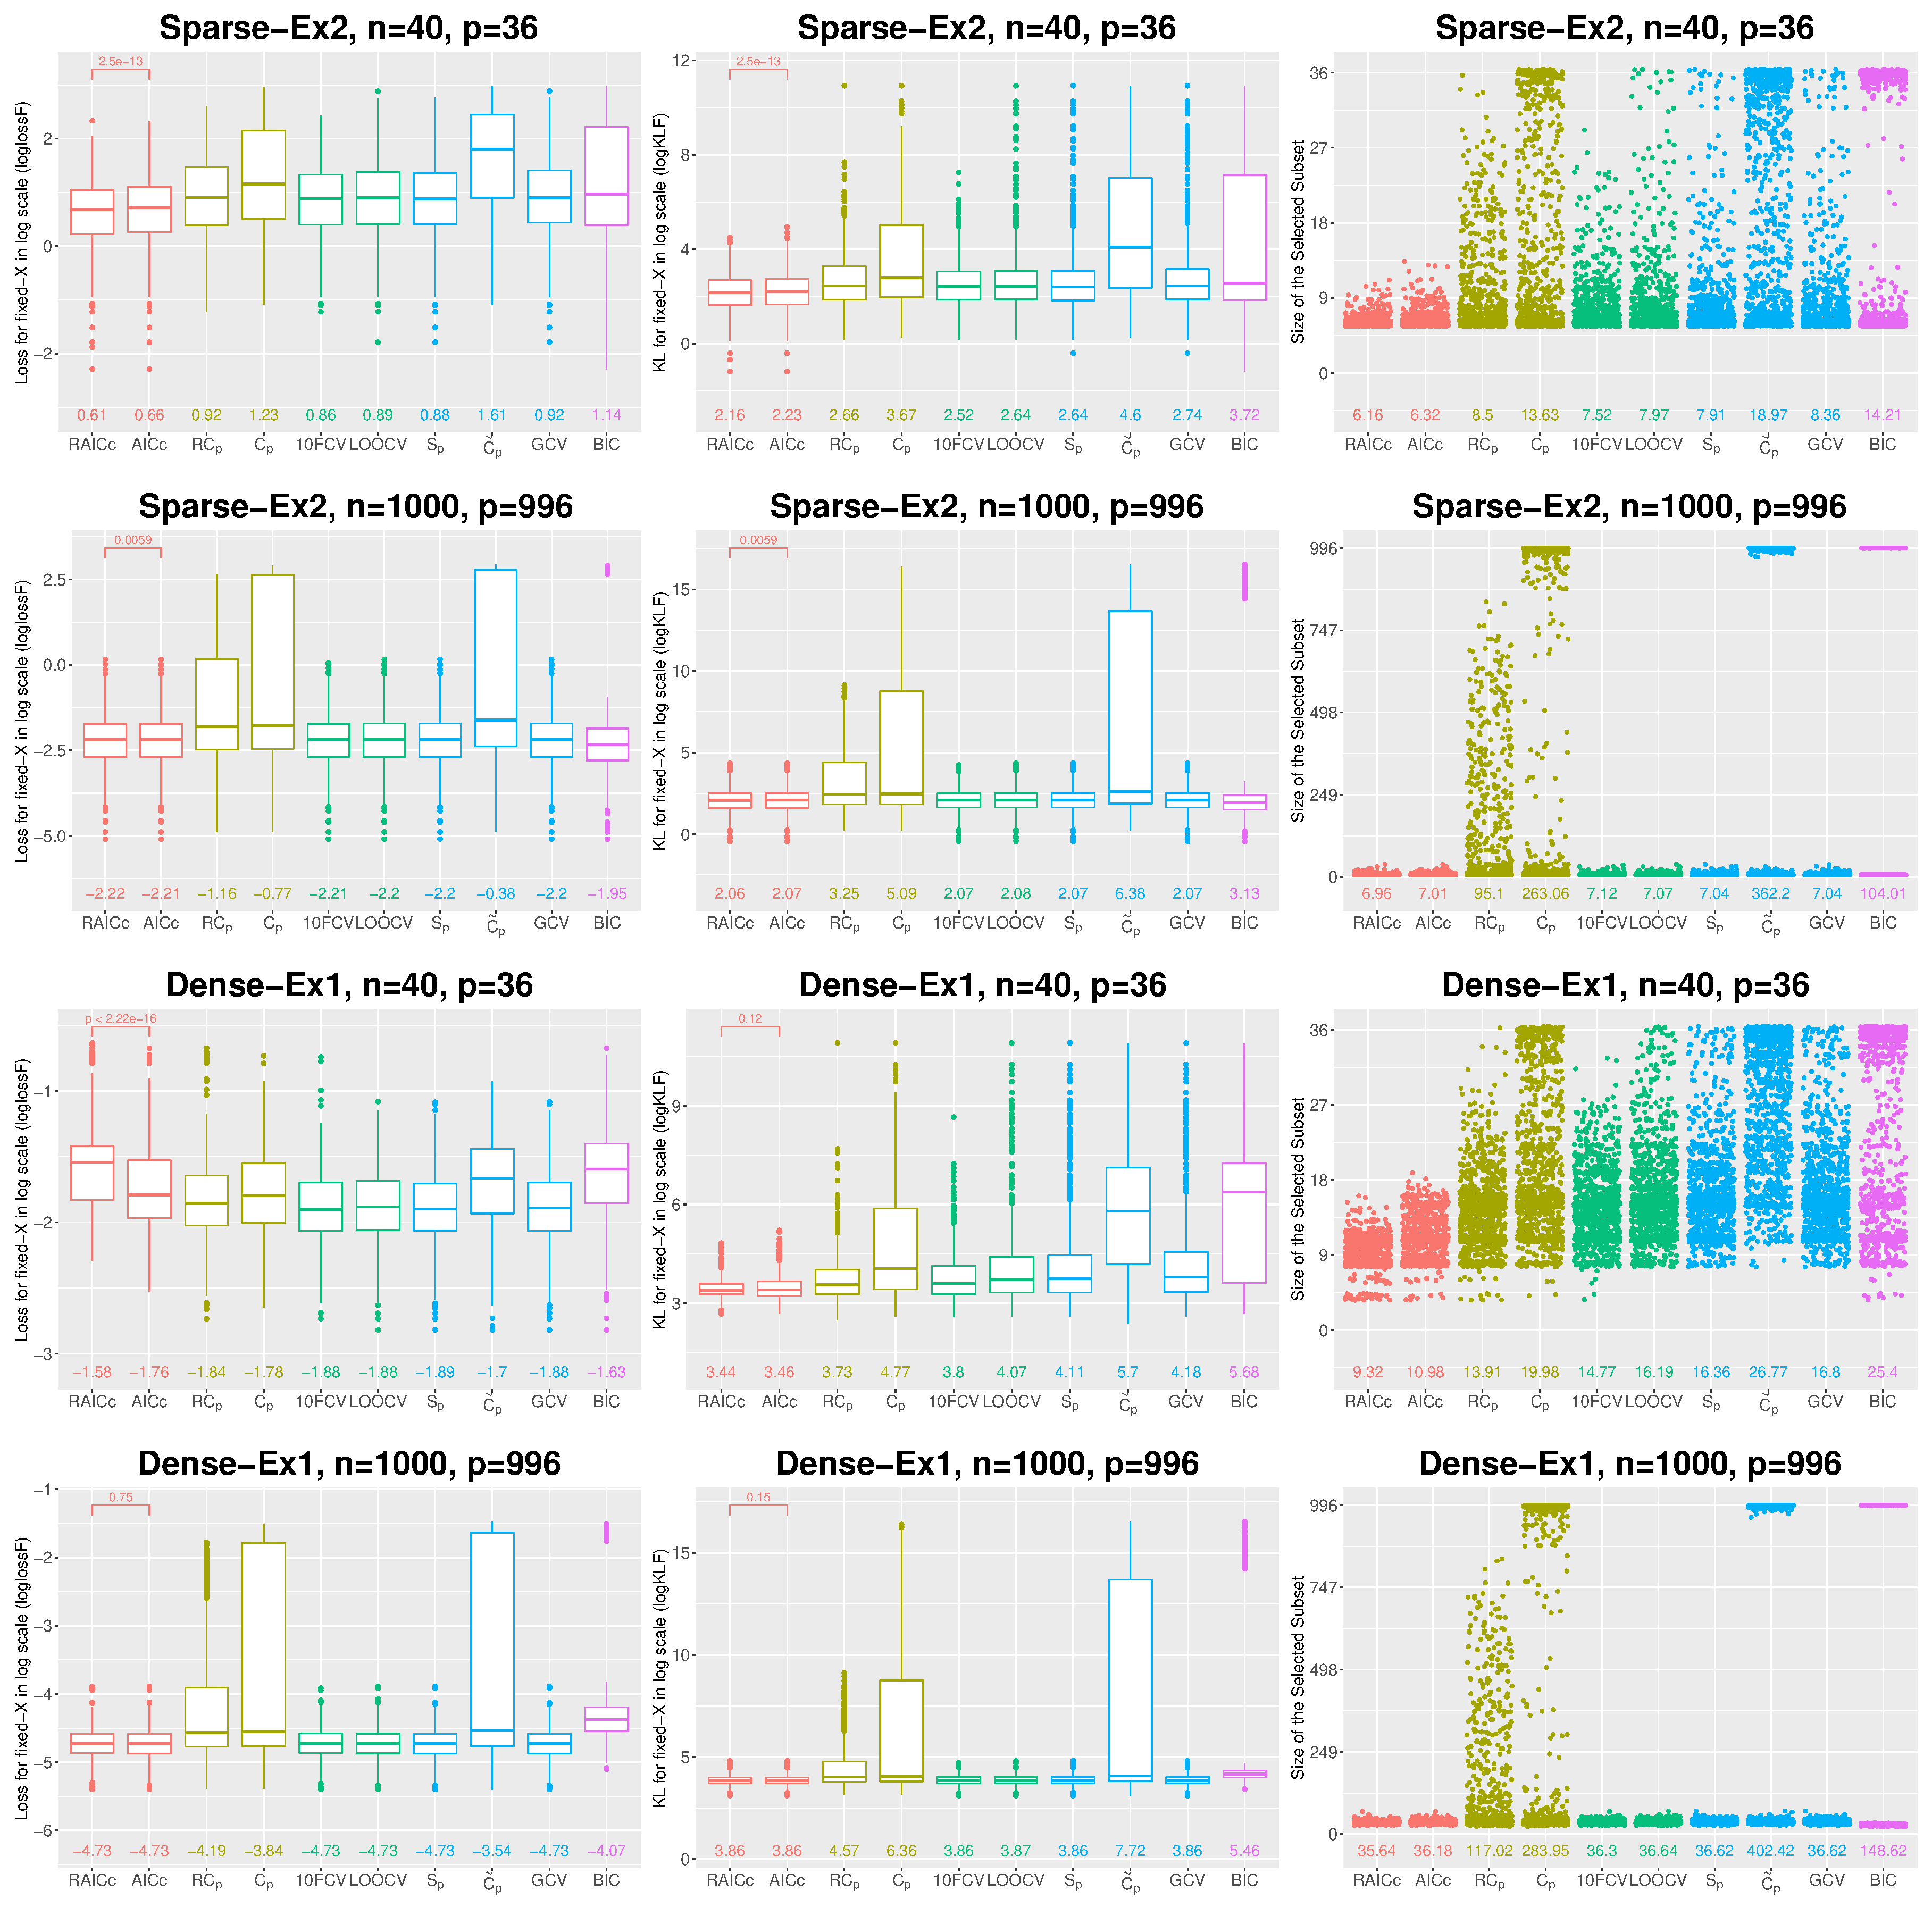
\includegraphics[width=\textwidth]{figures/main/fixedx/subset_selection/largep_hsnr.eps}
  \caption{Fixed-X, high signal and $\rho=0.5$. The mean values of the evaluation metrics for each criterion are presented at the bottom of each graph. The p-values of the Wilcoxon signed-rank test (paired and two-sided) for comparing RAICc and AICc are also presented.}
  \label{fig:subsetselection_fixedx_hsnr_largep}
\end{figure}


\begin{figure}[!ht]
  \centering
  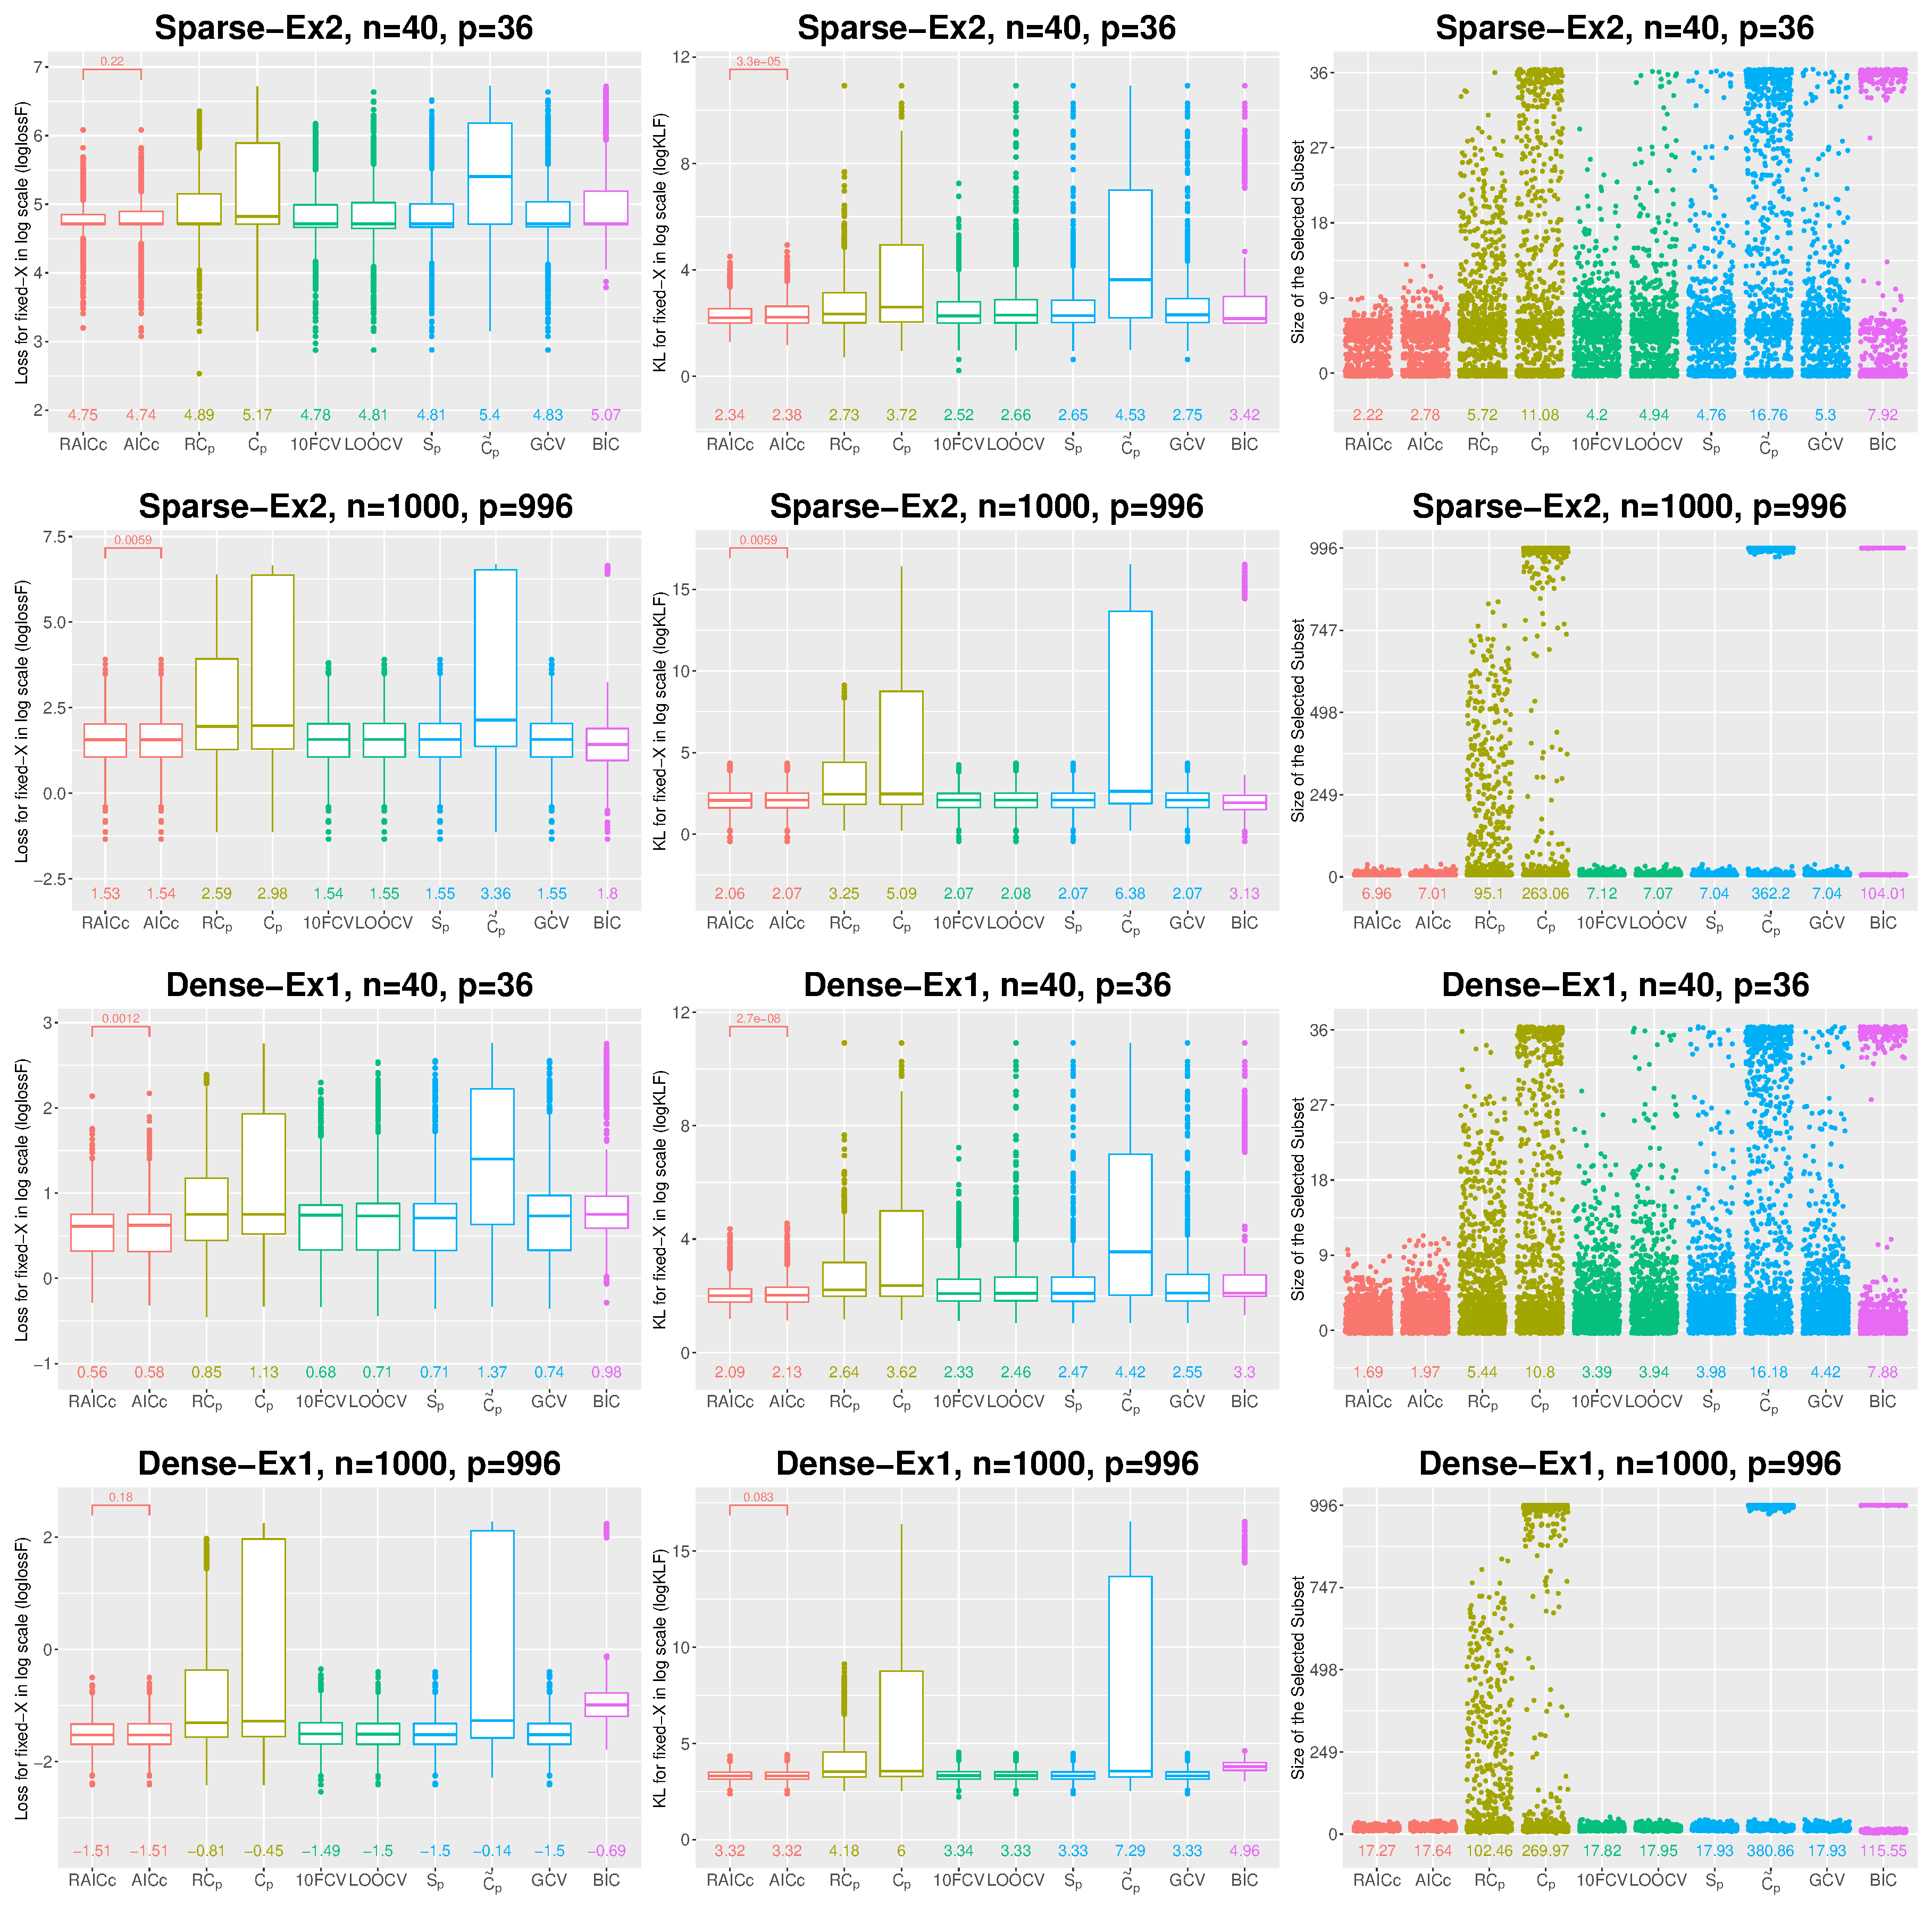
\includegraphics[width=\textwidth]{figures/main/fixedx/subset_selection/largep_lsnr.eps}
  \caption{Fixed-X, low signal and $\rho=0.5$. The mean values of the evaluation metrics for each criterion are presented at the bottom of each graph. The p-values of the Wilcoxon signed-rank test (paired and two-sided) for comparing RAICc and AICc are also presented.}
  \label{fig:subsetselection_fixedx_lsnr_largep}
\end{figure}

\begin{figure}[!ht]
  \centering
  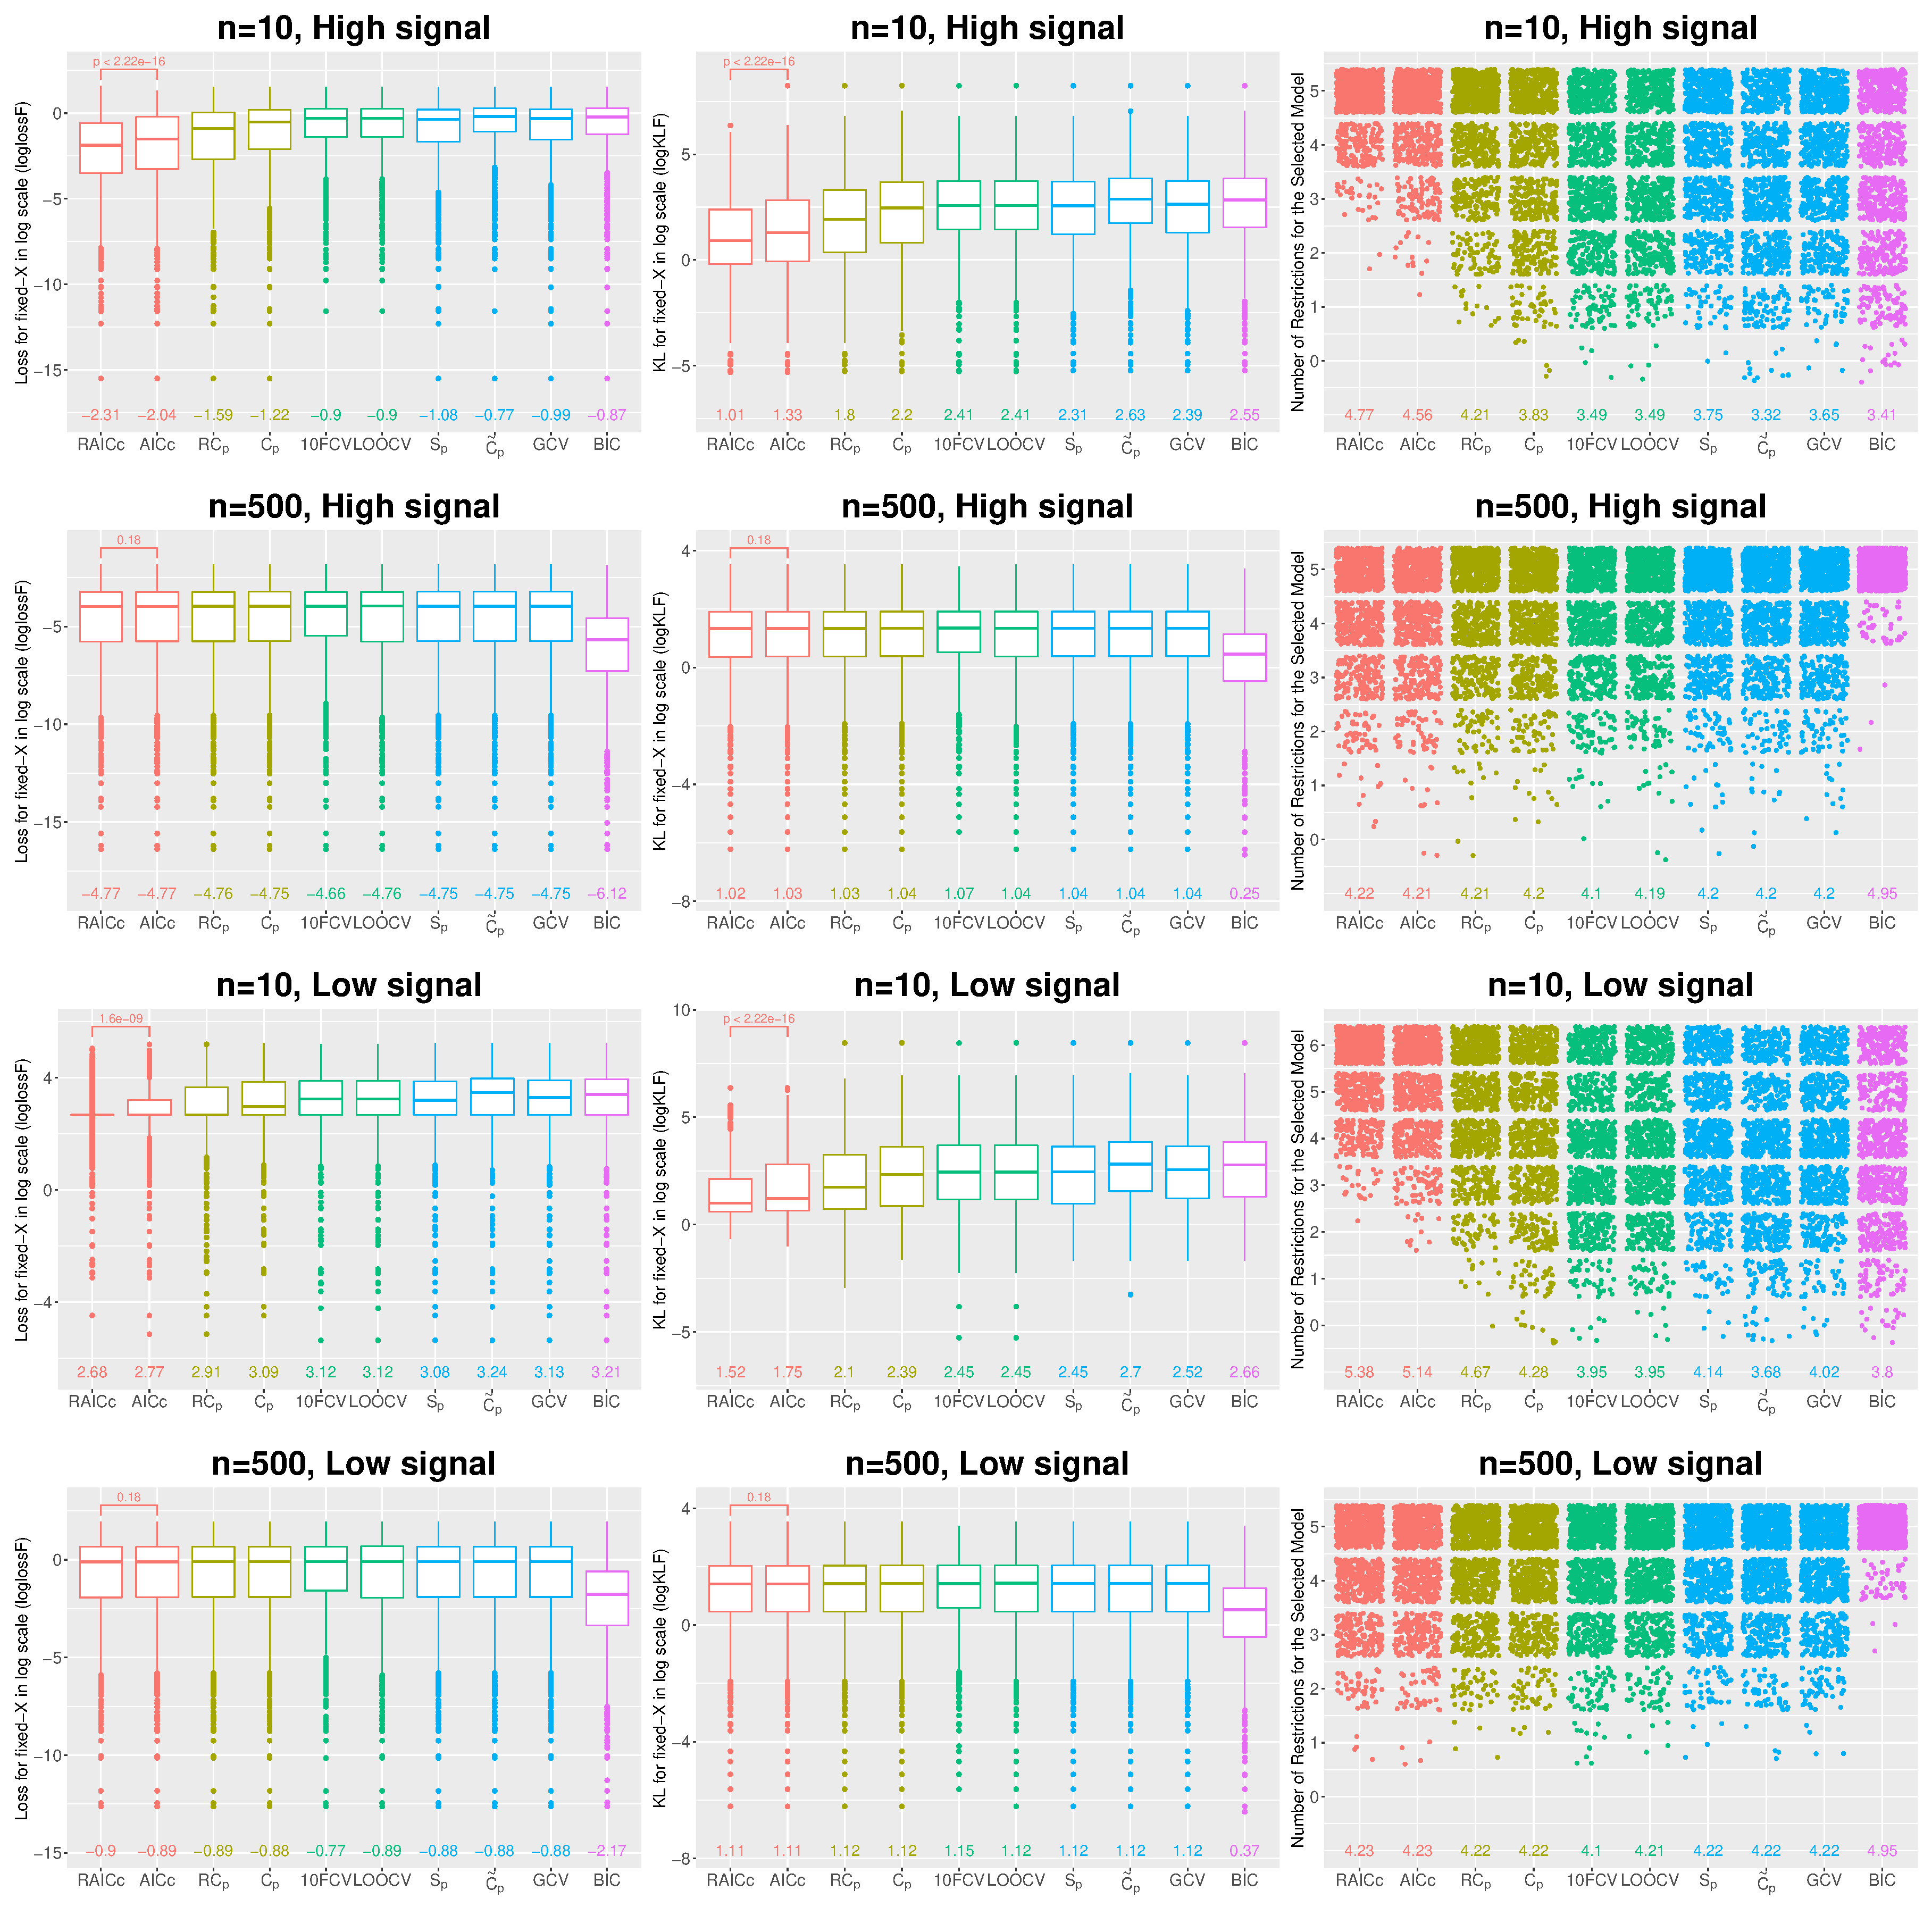
\includegraphics[width=\textwidth]{figures/main/fixedx/general_restriction/Ex1.eps}
  \caption{Fixed-X, Ex1, $p=6$, $\rho=0.5$. The mean values of the evaluation metrics for each criterion are presented at the bottom of each graph. The p-values of the Wilcoxon signed-rank test (paired and two-sided) for comparing RAICc and AICc are also presented.}
  \label{fig:generalrestriction_fixedx}
\end{figure}